\exercisesection{WITT 向量}

在习题 1 至 27 中，p 表示一个固定的素数。若 A 是一个环，则维特向量环 W(A) 指的是依附于素数 p 的那个维特向量环。

\begin{enumerate}
\def\labelenumi{\arabic{enumi})}
\item
  设 A 是一个环。加法群 W(A) 的自同态 V 能否与 W(A) 的乘法相容？
\item
  设 A 为环 \(\mathbf{Z}[(X_n)_{n\in\mathbb{N}}, (Y_n)_{n\in\mathbb{N}}]\)，即关于两个未定元族 \((X_n)\) 与 \((Y_n)\) 的多项式所成的环；又设 B 为环 \(\mathbf{Z}[X, Y]\)，即关于两个未定元 \(X\) 与 \(Y\) 的多项式所成的环。对每个多项式 \(R\)（属于 \(B\)），存在唯一的多项式序列 \((R_n)_{n\in\mathbb{N}}\)（各项属于 \(A\)），使得对每个 \(n\in\mathbb{N}\)，
\end{enumerate}

\[
\mathrm{R} \left(\Phi_ {n} \left(\mathrm{X} _ {0}, \dots , \mathrm{X} _ {n}\right), \Phi_ {n} \left(\mathrm{Y} _ {0}, \dots , \mathrm{Y} _ {n}\right)\right) = \Phi_ {n} \left(\mathrm{R} _ {0}, \dots , \mathrm{R} _ {n}\right).
\]

我们有 \(R_{0} = \mathrm{R}(X_{0}, Y_{0})\)，且 \(R_{n}\) 与 \(X_{i}\)、\(Y_{i}\)（当 i \textgreater{} n 时）无关。若 R 关于 X 是 r 次齐次的（相应地，关于 Y、关于 (X, Y) 是 r 次齐次的），并且对每个 \(i \in \mathbf{N}\) 赋予权重 \(p^{i}\) 于 \(X_{i}\) 与 \(Y_{i}\)，则 \(R_{n}\) 是权为 \(rp^{n}\) 的等权多项式——这里指关于 \((X_{i})_{i \in \mathbb{N}}\)（相应地，关于 \((Y_{i})_{i \in \mathbb{N}}\)，分别关于 \(((X_{i})_{i \in \mathbb{N}}, (Y_{i})_{i \in \mathbb{N}})\)）。若 R 是常数，则 \(R_{n}\) 是常数。试考察 R = 0, 1, -1, X + Y, XY, -X 诸情形。

\begin{enumerate}
\def\labelenumi{\arabic{enumi})}
\setcounter{enumi}{2}
\tightlist
\item
  \begin{enumerate}
  \def\labelenumii{\alph{enumii})}
  \tightlist
  \item
    存在唯一的多项式序列 \((\mathbf{R}_n)_{n\in \mathbb{N}}\)（各项属于 \(\mathbf{Z}[\mathrm{X},\mathrm{Y}]\)），使得对每个整数 \(n\geqslant 0\)，有
  \end{enumerate}
\end{enumerate}

\[
\mathrm{X} ^ {p ^ {n}} + \mathrm{Y} ^ {p ^ {n}} = \sum_ {i = 0} ^ {n} p ^ {i} \mathrm{R} _ {i} (\mathrm{X}, \mathrm{Y}) ^ {p ^ {n - i}}.
\]

\begin{enumerate}
\def\labelenumi{\alph{enumi})}
\setcounter{enumi}{1}
\tightlist
\item
  若 \(p\) 为奇数，则对一切 \(n \in \mathbf{N}\)，有
\end{enumerate}

\[
\mathrm{R} _ {n} (\mathrm{X}, - \mathrm{X}) = 0.
\]

若 \(p = 2\)，则有

\[
\mathrm{R} _ {1} (\mathrm{X}, \mathrm{Y}) = - \mathrm{XY}
\]

且有

\[
\mathrm{R} _ {n} (\mathrm{X}, \mathrm{X}) \equiv 0 \bmod . 2 \quad \text { for } \quad n \geqslant 2.
\]

\begin{enumerate}
\def\labelenumi{\arabic{enumi})}
\setcounter{enumi}{3}
\tightlist
\item
  设 A 是一个环，\(\boldsymbol{a} = (a_n)_{n \in \mathbb{N}}\) 是 W(A) 的一个元素，\(\boldsymbol{a}^{(p)}\) 是 W(A) 中的元素 \((a_n^p)_{n \in \mathbb{N}}\)。令
\end{enumerate}

\[
\boldsymbol {b} = (b _ {n}) _ {n \in \mathbb {N}} = p. \boldsymbol {a} - \mathrm{V} \boldsymbol {a} ^ {(p)}.
\]

证明我们有 \(b_n - pa_n \in p^{p-1} \mathbf{A}\)（对每个 \(n \in \mathbf{N}\)）。（化归为 \(\mathbf{A} = \mathbf{Z}[(\mathbf{X}_n)_{n \in \mathbb{N}}]\) 且 \(\boldsymbol{a} = (\mathbf{X}_n)_{n \in \mathbb{N}}\) 的情形，并利用 § 1, 第 1 目的命题 1。）

\begin{enumerate}
\def\labelenumi{\arabic{enumi})}
\setcounter{enumi}{4}
\tightlist
\item
  设 A 是特征为 \(p\) 的环。
\end{enumerate}

\begin{enumerate}
\def\labelenumi{\alph{enumi})}
\item
  环 W(A) 是整环当且仅当 A 是整环。
\item
  W(A) 是约化环当且仅当 A 是约化环。
\item
  下列条件等价：
\end{enumerate}

\begin{enumerate}
\def\labelenumi{(\roman{enumi})}
\item
  A 是特征 p 的完满环。
\item
  W(A)/pW(A) 是约化的。
\end{enumerate}

\begin{enumerate}
\def\labelenumi{\arabic{enumi})}
\setcounter{enumi}{5}
\item
  设 A 是一个 \(\mathbf{Z}_{(p)}\) -代数。设 n 为整数，\(n \geqslant 1\)，\(\boldsymbol{g} = (g_{0}, \ldots, g_{n-1})\) 是 \(\mathrm{W}_{n}(\mathrm{A})\) 的一个元素，且 \(f = g_{0}\)。若以 \(\mathrm{A}_{f}\)（相应地，\(\mathrm{W}_{n}(\mathrm{A})_{\boldsymbol{g}}\)）表示 A（相应地，\(\mathrm{W}_{n}(\mathrm{A})\)）关于 f 的幂（相应地，g 的幂）所成乘法系的局部化，则有 \(\mathrm{W}_{n}(\mathrm{A}_{f}) = \mathrm{W}_{n}(\mathrm{A})_{\boldsymbol{g}}\)。
\item
  设 A 是特征 \(p\) 的环。证明 W(A) 的 \(\mathcal{C}\) 拓扑与 \(p\) 进拓扑相重合当且仅当 A 是完满的。
\item
  设 A 是一个环，\(\xi\) 是 A 中满足 \(\sum_{i=0}^{p-1} \xi^i = 0\) 的元素。于是在 W(A) 中有等式
\end{enumerate}

\[
\mathrm{V} _ {\mathbf {A}} (\mathbf {1}) = \sum_ {i = 0} ^ {p - 1} \tau_ {\mathbf {A}} (\xi^ {i}).
\]

由此推出，若 A 的特征为 p，则有

\[
\mathrm{V} _ {\mathrm{A}} \circ \mathrm{F} _ {\mathrm{A}} (\boldsymbol {a}) = p. \boldsymbol {a} \quad \text { for all } \quad \boldsymbol {a} \in \mathrm{W} (\mathrm{A}).
\]

\begin{enumerate}
\def\labelenumi{\arabic{enumi})}
\setcounter{enumi}{8}
\item
  设 A 是特征 p 的域。证明环 W(A) 是诺特环当且仅当 A 是完满的。（计算向量空间 \(V_{1}(A)/V_{1}(A)^{2}\) 在 A 上的维数。）
\item
  设 \(k\) 是特征 \(p\) 的域，且具有有限的 \(p\) 基。设 A 是一个环，\(\varphi\) 是从 \(k\) 到 A 的同态，它使 A 成为 \(k\) 上的有限型代数。
\end{enumerate}

\begin{enumerate}
\def\labelenumi{\alph{enumi})}
\item
  对每个整数 \(n \geqslant 1\)，A 是 \(\mathbf{A}^{p^n}\) 上的有限生成模。
\item
  对每个整数 \(n \geqslant 1\)，\(\mathbf{W}_n(\mathbf{A})\) 是 \(\mathbf{W}_n(k)\) 上的有限型代数。
\end{enumerate}

（若 \(a_{1},\ldots,a_{N}\) 既作为 \(k\) -代数又作为 \(\mathbf{A}^{p^{n-1}}\) -模生成 A，试证元素 \(\mathrm{V}^j\tau(a_i)\)（\(1\leqslant i\leqslant N\)，\(0\leqslant j\leqslant n-1\)）生成 \(\mathrm{W}_{n}(k)\) -代数 \(\mathrm{W}_{n}(\mathbf{A})\)。）

\begin{enumerate}
\def\labelenumi{\arabic{enumi})}
\setcounter{enumi}{10}
\tightlist
\item
  设 A 是特征 p 的环。
\end{enumerate}

\begin{enumerate}
\def\labelenumi{\alph{enumi})}
\item
  设 \(n \in \mathbf{N}\)；证明有 \(p^{n-1}/n! \in \mathbf{Z}_{(p)}\)。证明 \((nm)!/n!(m!)^n\) 是整数，其中 \(n, m\) 取自 \(\mathbf{N}\)。
\item
  对 \(n \in \mathbf{N}\)，设 \(\gamma_{n}: \mathrm{V}_{1}(\mathrm{A}) \to \mathrm{W}(\mathrm{A})\) 为由下式定义的映射：
\end{enumerate}

\[
\begin{array}{l l} \gamma_ {n} (\mathrm{V} x) = 1 & \text { if } n = 0, \\ \gamma_ {n} (\mathrm{V} x) = (p ^ {n - 1} / n!) \mathrm{V} (x ^ {n}) & \text { if } n \geqslant 1. \end{array}
\]

\begin{enumerate}
\def\labelenumi{(\roman{enumi})}
\item
  证明我们有 \(\gamma_{n}(x)\in\mathbf{V}_{1}(\mathbf{A})\)（当 \(n\geqslant 1\) 且 \(x\in\mathbf{V}_{1}(\mathbf{A})\) 时）。
\item
  对 \(x, y \in \mathbf{V}_1(\mathbf{A})\) 与 \(n \in \mathbf{N}\)，有
\end{enumerate}

\[
\gamma_ {n} (x + y) = \sum_ {i = 0} ^ {n} \gamma_ {i} (x) \gamma_ {n - i} (y).
\]

\begin{enumerate}
\def\labelenumi{(\roman{enumi})}
\setcounter{enumi}{2}
\tightlist
\item
  对 \(\lambda \in \mathbf{W}(\mathbf{A}), x \in \mathbf{V}_1(\mathbf{A}), n \in \mathbf{N}\)，有
\end{enumerate}

\[
\gamma_ {n} (\lambda x) = \lambda^ {n} \gamma_ {n} (x).
\]

\begin{enumerate}
\def\labelenumi{(\roman{enumi})}
\setcounter{enumi}{3}
\tightlist
\item
  对 \(x \in \mathbf{V}_1(\mathbf{A})\) 与 \(n, m\)（属于 \(\mathbf{N}\)），有
\end{enumerate}

\[
\gamma_ {n} (x) \gamma_ {m} (x) = \binom {m + n} {n} \gamma_ {n + m} (x)
\]

以及

\[
\gamma_ {n} (\gamma_ {m} (x)) = \frac {(n m) !}{n ! (m !) ^ {n}} \gamma_ {n m} (x).
\]

\begin{enumerate}
\def\labelenumi{(\alph{enumi})}
\setcounter{enumi}{21}
\tightlist
\item
  我们有 \(\mathrm{F}\gamma_{n}(\mathrm{V}x) = (p^{n}/n!)x^{n}\) 与 \(\gamma_{n}(px) = (p^{n}/n!)x^{n}\)，其中 \(x \in \mathbf{W}(\mathbf{A})\)。
\end{enumerate}

\begin{enumerate}
\def\labelenumi{\arabic{enumi})}
\setcounter{enumi}{11}
\tightlist
\item
  设 A 是特征 \(p\) 的环。对每个元素 \(\boldsymbol{a} = (a_n)_{n \in \mathbb{N}}\)（属于 \(\mathrm{W(A)}\)）与每个整数 \(n \in \mathbb{N}\)，令 \(\boldsymbol{a}_+ = (a_{n+1})_{n \in \mathbb{N}}\)。
\end{enumerate}

\begin{enumerate}
\def\labelenumi{\alph{enumi})}
\item
  我们有 \(a = \tau(a_{0}) + V a_{+}\)。
\item
  以 \(\alpha : \mathrm{W}(\mathbf{A}) \to \mathrm{W}(\mathrm{A})\) 表示把 \(a = (a_n)_{n \in \mathbb{N}}\) 映为
\end{enumerate}

\[
\alpha (\boldsymbol {a}) = \boldsymbol {a} _ {+} - \sum_ {i = 1} ^ {p - 1} \frac {1}{p} \binom {p} {i} \tau (a _ {0}) ^ {p - i} (\mathrm{V} \boldsymbol {a} _ {+}) ^ {i} - (p - 1)! \gamma_ {p} (\mathrm{V} \boldsymbol {a} _ {+}),
\]

的映射，其中（参见上一习题）已令 \(\gamma_{p}(\mathrm{V}\boldsymbol{a}_{+}) = (p^{p-1}/p!)\mathrm{V}(\boldsymbol{a}_{+}^{p})\)。证明在 \(\mathbf{W}(\mathbf{A})\) 中有等式 \(\mathbf{F}\boldsymbol{a} = \boldsymbol{a}^{p} + p\alpha(\boldsymbol{a})\)。

\begin{enumerate}
\def\labelenumi{\alph{enumi})}
\setcounter{enumi}{2}
\tightlist
\item
  证明对每个整数 \(n \geqslant 1\)，\(\alpha\) 通过过渡到商定义了一个映射 \(\alpha_{n}\)，它从 \(\mathbf{W}_{n+1}(\mathbf{A})\) 映到 \(\mathbf{W}_{n}(\mathbf{A})\) 中。
\end{enumerate}

\begin{enumerate}
\def\labelenumi{\arabic{enumi})}
\setcounter{enumi}{12}
\tightlist
\item
  设 A 是特征 \(p\) 的环。W(A) 按理想 \(V_n(A)\) 的滤链与 W(A) 的环结构相容，以 gr \(_{V}\) (W(A)) 表示相应的相伴分次环。对每个整数 \(n \geqslant 0\)，我们用 \(\varphi_*^n A\) 表示赋以由同态 \(\varphi^n: A \to A\) 所给出的 A -代数结构的环 A，其中 \(\varphi\) 表示 \(p\) 次幂映射。证明对每个整数 \(n \geqslant 0\)，从 A 到 \(V_n(A)/V_{n+1}(A)\) 的、把 \(x \in A\) 映到 \(V^n\tau(x)\) 的类的映射，是 A -模 \(\varphi_*^n A\) 到 A -模 gr \(_{V}^n\) (W(A)) 上的同构。
\end{enumerate}

\[
\bigoplus_ {n \in \mathbf {N}} \varphi_ {*} ^ {n} \mathrm{A}
\]

\((x, y) \mapsto \varphi^{n} x. \varphi^{m} y \text{ 从 } \varphi_{*}^{m} A \times \varphi_{*}^{n} A \text{ 到 } \varphi_{*}^{m+n} A \text{ (对每对正整数 } (m, n)).\) 证明前面的诸同构定义了一个分次 A -代数同构 \(\bigoplus_{n\in \mathbf{N}}\varphi_{*}^{n} A \text{ 到 } gr_{V}(W(A))\)。

\begin{enumerate}
\def\labelenumi{\arabic{enumi})}
\setcounter{enumi}{13}
\tightlist
\item
  设 A 是一个环。假设 A 中乘以 \(p.1_{\mathrm{A}}\) 的映射是单射。设 \(\sigma\) 是 A 的一个自同态，满足 \(\sigma(x) \equiv x^p \mod p\mathrm{A}\)（对一切 \(x \in \mathrm{A}\)）。
\end{enumerate}

\begin{enumerate}
\def\labelenumi{\alph{enumi})}
\tightlist
\item
  存在唯一的从 A 到 W(A) 的环同态 \(s_{\sigma}\)，它满足
\end{enumerate}

\[
s _ {\sigma} \circ \sigma = F _ {A} \circ s _ {\sigma}
\]

以及

\[
\Phi_ {0} \circ s _ {\sigma} = \operatorname{Id} _ {\mathrm{A}}.
\]

  它也是从 A 到 W(A) 的唯一同态 \(s_{\sigma}\)，满足对每个正整数 \(n\) 有 \(\Phi_{n} \circ s_{\sigma} = \sigma^{n}\)。

\begin{enumerate}
\def\labelenumi{\alph{enumi})}
\setcounter{enumi}{1}
\item
  设 B 是一个环。假设 B 中乘以 \(p \cdot 1_{\mathbf{B}}\) 的映射是单射。设 \(\sigma'\) 是 B 的一个自同态，满足 \(\sigma'(x) \equiv x^p \mod p\mathbf{B}\)（对每个 \(x \in \mathbf{B}\)）。设 \(u\) 是从 A 到 B 的同态，满足 \(u \circ \sigma = \sigma' \circ u\)。则有 \(\mathbf{W}(u) \circ s_{\sigma} = s_{\sigma'} \circ u\)。
\item
  若以 \(t_{\sigma}\) 表示 \(s_{\sigma}\) 与 W(A) 到 W(A/pA) 上的典范投影的复合，证明 \(t_{\sigma}\) 对每个整数 \(n \geqslant 1\) 诱导一个同态 \(t_{\sigma,n}\)，它从 A/p \(^{n}\) A 映到 W \(_{n}\) (A/pA) 中。
\end{enumerate}

d) 若 A/pA 是完满的，证明 \(t_{\sigma,n}\) 是同构。（给 A 赋以理想 pA 的幂所成的滤链，并以 gr \(_{p}\) (A) 表示相应的相伴分次环，试证从 gr \(_{p}\) (A) 到 gr \(_{V}\) (W(A/pA)) 的、由 \(t_{\sigma}\) 诱导的同态（参见习题 13）是同构。）

\begin{enumerate}
\def\labelenumi{\alph{enumi})}
\setcounter{enumi}{4}
\tightlist
\item
  若 A/pA 是完满的，且 A 对 p 进拓扑是分离且完备的，则 \(t_{\sigma}\) 是从 A 到 W(A/pA) 上的同构。
\end{enumerate}

\begin{enumerate}
\def\labelenumi{\arabic{enumi})}
\setcounter{enumi}{14}
\tightlist
\item
  \begin{enumerate}
  \def\labelenumii{\alph{enumii})}
  \tightlist
  \item
    设 A 是一个环，使得 A 中乘以 \(p.1_{\mathbf{A}}\) 的映射是单射。则存在唯一的从 W(A) 到 W(W(A)) 的环同态 \(s_{\mathbf{A}}\)，满足
  \end{enumerate}
\end{enumerate}

\[
s _ {\mathbf {A}} \circ \mathrm{F} _ {\mathbf {A}} = \mathrm{F} _ {\mathbf {W} (\mathbf {A})} \circ s _ {\mathbf {A}}
\]

且有

\[
\Phi_ {0} \circ s _ {\mathrm{A}} = \operatorname{Id} _ {\mathrm{W(A)}}
\]

（\(\Phi_0\) 是 \(\mathbf{W}(\mathbf{W}(\mathbf{A}))\) 到 \(\mathbf{W}(\mathbf{A})\) 上的投影。它也是唯一的环同态，满足 \(\Phi_n\circ s_{\mathbf{A}} = \mathbf{F}_{\mathbf{A}}^{n}\)（对每个整数 \(n\in \mathbf{N}\)）（其中 \(\Phi_n:\mathbf{W}(\mathbf{W}(\mathbf{A}))\to \mathbf{W}(\mathbf{A})\) 是第 \(n\) 个幽灵分量，取值于 \(\mathbf{W}(\mathbf{W}(\mathbf{A}))\)）。

\begin{enumerate}
\def\labelenumi{\alph{enumi})}
\setcounter{enumi}{1}
\tightlist
\item
  考虑环 \(\mathcal{A} = \mathbf{Z}[(\mathrm{X}_n)_{n\in \mathbb{N}}]\)，即关于未定元族 \((\mathrm{X}_n)_{n\in \mathbb{N}}\) 的多项式所成的环。设 X 为元素 \((\mathrm{X}_n)_{n\in \mathbb{N}}\)（\(\mathrm{W}(\mathcal{A})\) 中的元素）。令 \(s_{\mathcal{A}}(\mathbf{X}) = (s_n(\mathbf{X}))_{n\in \mathbb{N}}\)，其中 \(s_n(\mathbf{X}) \in \mathrm{W}(\mathcal{A})\)。对每个环 A，定义从 W(A) 到 W(W(A)) 中的映射 \(s_{\mathbf{A}}\) 如下：\(s_{\mathbf{A}}(\boldsymbol{a}) = (s_{n}(\boldsymbol{a}))_{n \in \mathbb{N}}\)。证明 \(s_{\mathbf{A}}\) 是环同态，且满足
\end{enumerate}

\[
s _ {\mathbf {A}} \circ \mathbf {F} _ {\mathbf {A}} = \mathbf {F} _ {\mathbf {W} (\mathbf {A})} \circ s _ {\mathbf {A}}
\]

且有

\[
\Phi_ {0} \circ s _ {\mathrm{A}} = \operatorname{Id} _ {\mathrm{W(A)}}.
\]

\begin{enumerate}
\def\labelenumi{\alph{enumi})}
\setcounter{enumi}{2}
\tightlist
\item
  对每个环同态 \(u: \mathbf{B} \to \mathbf{A}\)，有
\end{enumerate}

\[
s _ {\mathrm{A}} \circ \mathrm{W} (u) = \mathrm{W} (\mathrm{W} (u)) \circ s _ {\mathrm{B}}.
\]

\begin{enumerate}
\def\labelenumi{\alph{enumi})}
\setcounter{enumi}{3}
\tightlist
\item
  映射 \(\mathbf{W}(s_{\mathbf{A}})\circ s_{\mathbf{A}}\) 与 \(s_{\mathbf{W(A)}}\circ s_{\mathbf{A}}\)（都是从 \(\mathbf{W}(\mathbf{A})\) 到 \(\mathbf{W}(\mathbf{W}(\mathbf{W}(\mathbf{A})))\) 中的映射）相等。
\end{enumerate}

\[
x \in \mathrm{A},
\]

\[
s _ {\mathbf {A}} \left(\tau_ {\mathbf {A}} (x)\right) = \tau_ {\mathbf {W} (\mathbf {A})} \left(\tau_ {\mathbf {A}} (x)\right).
\]

\begin{enumerate}
\def\labelenumi{\alph{enumi})}
\setcounter{enumi}{5}
\tightlist
\item
  我们有 \(s_{\mathrm{A}} \circ \mathrm{V}_{\mathrm{A}} = \mathrm{V}_{\mathrm{W(A)}} \circ s_{\mathrm{A}}\)，且映射 \(s_{\mathrm{A}}\) 当 W(A) 与 W(W(A)) 都赋以拓扑 \(\mathcal{G}\) 时是连续的。
\end{enumerate}

\begin{enumerate}
\def\labelenumi{\arabic{enumi})}
\setcounter{enumi}{15}
\tightlist
\item
  \begin{enumerate}
  \def\labelenumii{\alph{enumii})}
  \tightlist
  \item
    设 A、B 是两个环，\(\varphi\) 是从 A 到 B 的同态。则映射 \(\mathrm{W}(\varphi)\) 使集合 \(\mathrm{W(B)}\) 以及对一切 \(m \in \mathbf{N}\) 的集合 \(\mathrm{W}_{m}(\mathrm{B})\) 都得以赋以 \(\mathrm{W(A)}\) -模结构。若 \(m\)、\(n\) 是两个 \(\geqslant 0\) 的整数且 \(n \geqslant m\)，则从 \(\mathrm{W}_{n}(\mathrm{B})\) 到 \(\mathrm{W}_{m}(\mathrm{B})\) 上的典范映射是 \(\mathrm{W(A)}\) -线性的。此外，\(\mathrm{W(B)}\)（作为 \(\mathrm{W(A)}\) -模）是诸 \(\mathrm{W}_{m}(\mathrm{B})\) 的投影极限。
  \end{enumerate}
\end{enumerate}

\begin{enumerate}
\def\labelenumi{\alph{enumi})}
\setcounter{enumi}{1}
\tightlist
\item
  设 A、B 是两个环，\(\psi\) 是从 W(A) 到 B 的同态。令 \(\tilde{\psi} = \mathbf{W}(\psi) \circ s_{\mathbf{A}}\)（参见习题 15）。从 W(A) 到 W(B) 的映射 \(\tilde{\psi}\) 使集合 W(B) 以及对每个 \(m \in \mathbf{N}\) 的集合 W \(_{m}\) (B) 都得以赋以 W(A) -模结构，且 a) 中最后两个断言仍然成立。若 \(\varphi\) 是从 A 到 B 的同态且满足 \(\psi = \varphi \circ \Phi_{0}\)，则有 \(\tilde{\psi} = \mathbf{W}(\varphi)\)。
\end{enumerate}

\begin{enumerate}
\def\labelenumi{\arabic{enumi})}
\setcounter{enumi}{16}
\tightlist
\item
  设 A 是环 \(\mathbf{Q}[\mathbf{X}]\)。设 \(\boldsymbol{\Omega} = (\Omega_n)_{n \in \mathbb{N}}\) 是 \(\mathrm{W}(\mathrm{A})\) 中满足 \(\Phi_{\mathbf{A}}(\boldsymbol{\Omega}) = (\mathbf{X}, \mathbf{X}, ..., \mathbf{X}, ...)\) 的元素。对每个元素 \(a\)（属于 \(\mathbf{Z}_p\)），令
\end{enumerate}

\[
\boldsymbol {\Omega} (a) = \left(\Omega_ {n} (a)\right) _ {n \in \mathbf {N}}.
\]

\begin{enumerate}
\def\labelenumi{\alph{enumi})}
\item
  对每个 \(a \in \mathbf{Z}_p\) 与每个整数 \(n \in \mathbb{N}\)，有 \(\Omega_n(a) \in \mathbf{Z}_p\)。
\item
  对每个 \(a \in \mathbf{Z}\) 与每个整数 \(n \in \mathbf{N}\)，有 \(\Omega_n(a) \in \mathbf{Z}\)，且当 \(a \in \mathbf{N}\) 时，\(\Omega(a)\) 是 \(\mathbf{W}(\mathbf{Z})\) 中 \(a\) 个都等于 \(\mathbf{W}(\mathbf{Z})\) 的单位元的项之和。
\item
  映射 \(a \mapsto \Omega(a)\) 定义了一个从 \(\mathbf{Z}_{p}\) 到 \(\mathrm{W}(\mathbf{Z}_{p})\) 的同态，当把 \(\mathbf{Z}_{p}\) 与 \(\mathrm{W}(\mathbf{F}_{p})\) 等同看待时（\(\S\) 1, 第 7 目，例 3），该同态与习题 15 中定义的同态 \(s_{\mathbf{F}_{p}}\) 相重合。
\end{enumerate}

\begin{enumerate}
\def\labelenumi{\arabic{enumi})}
\setcounter{enumi}{17}
\tightlist
\item
  \begin{enumerate}
  \def\labelenumii{\alph{enumii})}
  \tightlist
  \item
    设 L 是一个（交换）域。设 G 是 L 的一个自同构群，K 是 G 的不变量域。则 G 的每个元素 g 都（经由 W(g)）作用在 W(L) 上，且对每个整数 \(n \geqslant 1\)，也作用在 \(W_{n}(L)\) 上。W(L)（相应地，\(W_{n}(L)\)）中在 G 的作用下不变的元素所成的集合是 W(K)（相应地，\(W_{n}(K)\)）。
  \end{enumerate}
\end{enumerate}

\begin{enumerate}
\def\labelenumi{\alph{enumi})}
\setcounter{enumi}{1}
\tightlist
\item
  假设 L 是 K 的有限伽罗瓦扩张，并以 \(\mathbf{Z}[G]\) 表示（有限）群 G 在 \(\mathbf{Z}\) 上的代数。对每个 \(\mathbf{Z}\) -模 M，以 \(M^{G}\) 表示 \(\mathbf{Z}[G]\) -模 \(\operatorname{Hom}_{\mathbf{Z}}(\mathbf{Z}[G], M)\)（赋以其自然的左 \(\mathbf{Z}[G]\) -模结构）。证明 \(\mathbf{Z}[G]\) -模 W(L)（相应地，W \(_{n}\) (L)）同构于 W(K) \(^{G}\)（相应地，W \(_{n}\) (K) \(^{G}\)）。由此推出我们有
\end{enumerate}

\[
\mathrm{H} ^ {i} (\mathrm{G}, \mathrm{W} (\mathrm{L})) = 0 \quad (\text { resp. } \mathrm{H} ^ {i} (\mathrm{G}, \mathrm{W} _ {n} (\mathrm{L})) = 0)
\]

对每个整数 \(i > 0\)。（利用正规基定理，见 A, V, 第 70 页，定理 6 以及 A, X, 第 111 至 113 页。）

\begin{enumerate}
\def\labelenumi{\arabic{enumi})}
\setcounter{enumi}{18}
\tightlist
\item
  设 K 是特征为 p 的域，P 是它的素子域，Ω 是 K 的一个代数闭包。我们以 \(\wp\) 表示自同态 \(x \mapsto Fx - x\)（群 \(\mathrm{W}(\Omega)\) 的自同态），并且对每个整数 \(n \geqslant 1\)，也以它表示该自同态通过过渡到商而在 \(\mathrm{W}_{n}(\Omega)\) 上诱导的自同态。
\end{enumerate}

\begin{enumerate}
\def\labelenumi{\alph{enumi})}
\tightlist
\item
  我们固定一个整数 \(n \geqslant 1\)。\(\wp\) 作为 \(\mathrm{W}(\Omega)\)（相应地，\(\mathrm{W}_{n}(\Omega)\)）的自同态，保持 \(\mathrm{W}(\mathrm{K})\)（相应地，\(\mathrm{W}_{n}(\mathrm{K})\)）稳定，其核为 \(\mathrm{W}(\mathrm{P})\)（相应地，\(\mathrm{W}_{n}(\mathrm{P})\)）。
\end{enumerate}

在本习题的余下部分，我们将把 \(\mathbf{W}(\mathbf{P})\) 与 \(\mathbf{Z}_p\)、\(\mathbf{W}_n(\mathbf{P})\) 与 \(\mathbf{Z}/p^n\mathbf{Z}\) 等同看待（\(\S 1\)，第 7 目，例 3）。

\begin{enumerate}
\def\labelenumi{\alph{enumi})}
\setcounter{enumi}{1}
\item
  设 \(\boldsymbol{a} \in W_n(\mathbf{K})\)。以 V 表示位移同态 \(W_n(\mathbf{K}) \to W_{n+1}(\mathbf{K})\)，证明 \(\boldsymbol{a} \in \wp W_n(\mathbf{K})\) 当且仅当 \(Va \in \wp W_{n+1}(\mathbf{K})\)。若 K 是可分闭的，则有 \(\wp W_n(\mathbf{K}) = W_n(\mathbf{K})\)。
\item
  设 \(\pmb{a} \in \mathbf{W}_n(\Omega)\) 满足 \(\wp \pmb{a} \in \mathbf{W}_n(\mathbf{K})\)。我们以 \(\mathbf{K}(\pmb{a})\) 表示 \(\Omega\) 的由 \(\mathbf{K}\) 与分量 \(a_0, \ldots, a_{n-1}\)（\(\pmb{a}\) 的分量）生成的子域。若 \(\mathbf{A}\) 是 \(\mathbf{W}_n(\mathbf{K})\) 的一个子集，则以 \(\mathbf{K}(\wp^{-1}(\mathbf{A}))\) 表示 \(\Omega\) 的由诸域 \(\mathbf{K}(\pmb{a})\)（其中 \(\pmb{a}\) 取遍 \(\mathbf{W}_n(\Omega)\) 中满足 \(\wp \pmb{a} \in \mathbf{A}\) 的元素）生成的子扩张。
\end{enumerate}

仿照 A, V, 第 87 页的推理并利用前一习题，证明以下断言：

\begin{enumerate}
\def\labelenumi{(\roman{enumi})}
\tightlist
\item
  设 L 是 K 在 Ω 中的伽罗瓦扩张。存在唯一的映射 \((\sigma, a) \mapsto [\sigma, a]\)，它从 \(\operatorname{Gal}(\mathrm{L}/\mathrm{K}) \times (\wp W_{n}(\mathrm{L}) \cap W_{n}(\mathrm{K}))/\wp W_{n}(\mathrm{K})\) 映到 \(Z/p^{n}Z\) 中，使得对每个 \(\sigma \in \operatorname{Gal}(\mathrm{L}/\mathrm{K})\) 与每个 \(x \in W_{n}(\mathrm{L})\)（满足 \(\wp(x) \in W_{n}(\mathrm{K})\)），若以 \(\wp(x)\) 表示 \(\wp(x)\) 模 \(\wp W_{n}(\mathrm{K})\) 的类，则有
\end{enumerate}

\[
[ \sigma , \overline {{\wp (x)}} \rangle = \sigma x - x.
\]

若 \(\sigma, \sigma' \in \operatorname{Gal}(\mathbf{L} / \mathbf{K})\) 且 \(a, a' \in (\wp \mathrm{W}_n(\mathbf{L}) \cap \mathrm{W}_n(\mathbf{K})) / \wp \mathrm{W}_n(\mathbf{K})\)，则有

\[
[ \sigma \sigma^ {\prime}, a \rangle = [ \sigma , a \rangle + [ \sigma^ {\prime}, a \rangle
\]

以及

\[
[ \sigma , a + a ^ {\prime} \rangle = [ \sigma , a \rangle + [ \sigma , a ^ {\prime} \rangle .
\]

\begin{enumerate}
\def\labelenumi{(\roman{enumi})}
\setcounter{enumi}{1}
\tightlist
\item
  对 K 在 Ω 中的每个伽罗瓦扩张 L，记
\end{enumerate}

\[
a _ {\mathrm{L}}: (\wp \mathrm{W} _ {n} (\mathrm{L}) \cap \mathrm{W} _ {n} (\mathrm{K})) / \wp \mathrm{W} _ {n} (\mathrm{K}) \rightarrow \operatorname{Hom} (\operatorname{Gal} (\mathrm{L} / \mathrm{K}), \mathbf {Z} / p ^ {n} \mathbf {Z})
\]

与

\[
a _ {\mathrm{L}} ^ {\prime}: \operatorname{Gal} (\mathrm{L} / \mathrm{K}) \rightarrow \operatorname{Hom} ((\wp \mathrm{W} _ {n} (\mathrm{L}) \cap \mathrm{W} _ {n} (\mathrm{K})) / \wp \mathrm{W} _ {n} (\mathrm{K}), \mathbf {Z} / p ^ {n} \mathbf {Z})
\]

为 (i) 中定义的映射 \((\sigma, a) \mapsto [\sigma, a \rangle\) 所诱导的同态。对 K 在 \(\Omega\) 中的任意伽罗瓦扩张 L，同态 \(a_{L}\) 是单射，其像是由拓扑群 \(\operatorname{Gal}(\mathbf{L}/\mathbf{K})\) 到离散群 \(\mathbf{Z}/p^{n}\mathbf{Z}\) 的连续同态所成的群。

\begin{enumerate}
\def\labelenumi{(\roman{enumi})}
\setcounter{enumi}{2}
\item
  映射 \(\mathbf{A} \mapsto \mathbf{K}(\wp^{-1}(\mathbf{A}))\) 是从 \(\mathrm{W}_n(\mathbf{K})\) 的包含 \(\wp\mathrm{W}_n(\mathbf{K})\) 的子群全体到 \(\mathbf{K}\) 在 \(\Omega\) 中的、在 \(\mathbf{K}\) 上交换且指数整除 \(p^n\) 的扩张全体上的双射。其逆映射为 \(\mathrm{L} \mapsto \wp\mathrm{W}_n(\mathrm{L}) \cap \mathrm{W}_n(\mathbf{K})\)。
\item
  对 \(\mathbf{W}_{n}(\mathbf{K})\) 的每个包含 \(\wp\mathbf{W}_{n}(\mathbf{K})\) 的子群 A，同态
\end{enumerate}

\[
a _ {\mathrm{K} (\wp ^ {- 1} (\mathrm{A}))} ^ {\prime}: \operatorname{Gal} \left(\mathrm{K} \left(\wp ^ {- 1} (\mathrm{A})\right) / \mathrm{K}\right)\rightarrow \operatorname{Hom} \left(\mathrm{A} / \wp \mathrm{W} _ {n} (\mathrm{K}), \mathrm{Z} / p ^ {n} \mathrm{Z}\right)
\]

是双射的。当给 \(\operatorname{Hom}(\mathbf{A}/\wp\mathbf{W}_n(\mathbf{K}), \mathbf{Z}/p^n\mathbf{Z})\) 赋以逐点收敛拓扑时，它是一个同胚。

\begin{enumerate}
\def\labelenumi{\arabic{enumi})}
\setcounter{enumi}{19}
\tightlist
\item
  我们保留前一习题的假设与记号。
\end{enumerate}

\begin{enumerate}
\def\labelenumi{\alph{enumi})}
\tightlist
\item
  对 K 在 \(\Omega\) 中的每个扩张 L，考虑 \(\bar{Z}_{p}\) -模
\end{enumerate}

\[
\mathfrak {W} (\mathrm{L}) = \left(\mathrm{W} (\mathrm{L}) / p \mathrm{W} (\mathrm{L})\right) \otimes_ {\mathbf {Z} _ {p}} \left(\mathbf {Q} _ {p} / \mathbf {Z} _ {p}\right)
\]

以及对每个整数 \(n \geqslant 0\)，其子模

\[
\mathcal {W} _ {n} (\mathrm{L}) = \left(\mathrm{W} (\mathrm{L}) / \wp \mathrm{W} (\mathrm{L})\right) \otimes_ {\mathbf {Z} _ {p}} \left(p ^ {- n} \mathbf {Z} _ {p} / \mathbf {Z} _ {p}\right).
\]

证明 \(\mathcal{W}(\mathbf{L})\) 等同于其子模 \(\mathcal{W}_{n}(\mathbf{L})\) 关于下列包含映射的归纳极限：

\[
i _ {n}: \mathcal {W} _ {n} (\mathrm{L}) \rightarrow \mathcal {W} _ {n + 1} (\mathrm{L}).
\]

\begin{enumerate}
\def\labelenumi{\alph{enumi})}
\setcounter{enumi}{1}
\tightlist
\item
  对每个整数 \(n \geqslant 0\)，设 \(\psi_n\) 是从 \(\mathfrak{W}_n(L)\) 到 \(\mathrm{W}_n(L)/p\mathrm{W}_n(L)\) 的、把 \(x \otimes p^{-n}\) 映为 \(x\) 的类的映射。证明 \(\psi_n\) 是同构且有
\end{enumerate}

\[
\mathrm{V} _ {n} \circ \psi_ {n} = \psi_ {n + 1} \circ i _ {n},
\]

其中 \(V_{n}\) 是由位移 V 诱导的、从 \(\mathbf{W}_{n}(\mathbf{L})/\wp\mathbf{W}_{n}(\mathbf{L})\) 到 \(\mathbf{W}_{n+1}(\mathbf{L})/\wp\mathbf{W}_{n+1}(\mathbf{L})\) 的映射。由此推出 \(\mathfrak{W}(\mathbf{L})\) 可与群 \(\mathbf{W}_{n}(\mathbf{L})/\wp\mathbf{W}_{n}(\mathbf{L})\) 沿映射 \(V_{n}\) 的归纳极限等同。

\begin{enumerate}
\def\labelenumi{\alph{enumi})}
\setcounter{enumi}{2}
\tightlist
\item
  设 \(a \in \mathcal{W}(\mathbf{K})\)。若 \(n\) 是使 \(a\) 属于 \(\mathcal{W}_n(\mathbf{K})\) 的整数，则我们在习题 19, c) 中已经构造了扩张 \(\mathbf{K}(\wp^{-1}(\psi_n(a)))\)。这一扩张不依赖于整数 \(n\) 的选取；我们把它记作 \(\mathbf{K}(\wp^{-1}(a))\)。若 A 是 \(\mathcal{W}(\mathbf{K})\) 的一个子集，我们以 \(\mathbf{K}(\wp^{-1}(\mathbf{A}))\) 表示由诸域 \(\mathbf{K}(\wp^{-1}(a))\)（当 \(a\) 取遍 A 时）生成的扩张。证明 \(\mathbf{K}(\wp^{-1}(\mathbf{A}))\) 是 K 的一个交换扩张。在此情形下证明与习题 19, c) 中断言 (i) 至 (iv) 类似的断言。
\end{enumerate}

\begin{enumerate}
\def\labelenumi{\arabic{enumi})}
\setcounter{enumi}{20}
\tightlist
\item
  我们保留前两个习题的假设与记号。
\end{enumerate}

\begin{enumerate}
\def\labelenumi{\alph{enumi})}
\item
  乘以 \(p\) 在 \(\mathbf{W}(\mathbf{K}) / p\mathbf{W}(\mathbf{K})\) 中是单射。
\item
  设 \(\pmb{a}\) 是 \(\mathbf{W}(\Omega)\) 中满足 \(\pmb{a} \notin \mathbf{W}(\mathbf{K})\) 且 \(\wp \pmb{a} \in \mathbf{W}(\mathbf{K})\) 的元素。我们以 \(\mathrm{K}(\pmb{a})\) 表示 \(\Omega\) 的在 \(\mathbf{K}\) 上由分量 \((a_n)_{n \in \mathbb{N}}\)（\(\pmb{a}\) 的分量）生成的子域。证明 \(\mathrm{K}(\pmb{a})\) 是 \(\mathbf{K}\) 的交换扩张，其伽罗瓦群同构于拓扑群 \(\mathbf{Z}_p\)。
\item
  若 A 是 W(K) 的一个子集，则以 K( \(\wp^{-1}(A)\) ) 表示 Ω 的由诸域 K(a)（其中 a 取遍 W(Ω) 中满足 \(\wp a \in A\) 的元素）生成的子扩张。在此情形下证明与习题 19, c) 的断言 (i) 至 (iv) 类似的断言。
\end{enumerate}

\(d\) ) 设 \(\Gamma\) 是 \(\Omega\) 在 K 上的自同构群。设 \(n\) 是一个 \(\geqslant 1\) 的整数，\(\varphi_{n}\) 是 \(\Gamma\) 到 \(\mathbf{Z} / p^{n}\mathbf{Z}\) 中的连续同态。证明存在连续同态 \(\varphi\)（\(\Gamma\) 到 \(\mathbf{Z}_{p}\) 中的连续同态），它通过过渡到商诱导出 \(\varphi_{n}\)。若以 \(\mathrm{Hom}_c(\Gamma, \Gamma')\) 表示 \(\Gamma\) 到 \(\Gamma'\)（\(\Gamma'\) 为拓扑群）中的连续同态所成的群，证明典范映射

\[
\operatorname{Hom} _ {c} (\Gamma , \mathbf {Z} _ {p}) \otimes_ {\mathbf {Z} _ {p}} (\mathbf {Q} _ {p} / \mathbf {Z} _ {p}) \rightarrow \operatorname{Hom} _ {c} (\Gamma , \mathbf {Q} _ {p} / \mathbf {Z} _ {p})
\]

是同构。

\begin{enumerate}
\def\labelenumi{\arabic{enumi})}
\setcounter{enumi}{21}
\tightlist
\item
  设 A 是一个 \(\mathbf{Z}_{(p)}\) -代数。我们以 \(D_{A}\) 表示 W(A) 上由两个未定元 F 和 V 生成的、且满足下列关系式的代数
\end{enumerate}

\[
\begin{array}{l l l l} \mathbf {F a} & = (\mathbf {F a}). \mathbf {F} & \text { for } & a \in \mathbf {W} (\mathbf {A}) \\ a \mathbf {V} & = \mathbf {V} (\mathbf {F a}) & \text { for } & a \in \mathbf {W} (\mathbf {A}) \\ \mathbf {F V} & = p & & \\ \mathbf {V a F} & = \mathbf {V a} & \text { for } & a \in \mathbf {W} (\mathbf {A}), \end{array}
\]

其中 F 与 V 分别表示 W(A) 的弗罗贝尼乌斯同态与位移同态。a) 设 B 是一个 A -代数。让 F 与 V 经由 W(B) 的弗罗贝尼乌斯同态与位移同态作用在 W(B) 上，我们就给 W(B) 赋以 \(\mathfrak{D}_{\mathrm{A}}\) -模结构。类似地，对每个整数 \(n \geqslant 1\)，W \(_n\) (B) 是一个 \(\mathfrak{D}_{\mathrm{A}}\) -模。

\begin{enumerate}
\def\labelenumi{\alph{enumi})}
\setcounter{enumi}{1}
\tightlist
\item
  对每个元素 \(x\)（属于 \(\mathfrak{D}_{\mathbf{A}}\)），存在 W(A) 的元素的一个有限支撑族 \((a_{i})_{i\in\mathbf{Z}}\)，由下列等式所刻画
\end{enumerate}

\[
x = \sum_ {n \geqslant 1} a _ {- n} \mathbf {F} ^ {n} + a _ {0} + \sum_ {n \geqslant 1} \mathbf {V} ^ {n} a _ {n}.
\]

\begin{enumerate}
\def\labelenumi{\alph{enumi})}
\setcounter{enumi}{2}
\item
  假设 W(A) 是整环。设 \(x \in \mathfrak{D}_{\mathbf{A}}\)。我们以 \(\delta(x)\) 表示最大的整数 \(n\)，使得 \(a_{n}\) 非零。若 \(x\) 与 \(y\) 是 \(\mathfrak{D}_{\mathbf{A}}\) 的两个非零元素，则有 \(\delta(xy) = \delta(x) + \delta(y)\)。由此推出 \(\mathfrak{D}_{\mathbf{A}}\) 是整环。
\item
  若 A 是特征为 p 的完满环，则可把条件 VaF = Va（\(a \in \mathrm{W}(\mathrm{A})\)）换成条件 VF = p。左理想 \(D_{A}V\)（\(D_{A}\) 中的左理想）是双边理想。
\item
  若 k 是特征为 p 的完满域，则 \(D_{k}\) 是诺特环。（把 \(D_{k}\) 看作 W(k) 上由两个未定元 X 与 Y 生成的、且满足关系式 XY = YX 与 Xa = (Fa) X, aY = Y(Fa)（\(a \in \mathrm{W}(k)\)）的环的一个商。然后应用 III, § 2, 第 8 目，定理 1 的推论 2 以及习题 10。）
\end{enumerate}

\begin{enumerate}
\def\labelenumi{\arabic{enumi})}
\setcounter{enumi}{22}
\tightlist
\item
  设 A 是一个环，I 是负整数的集合。设 m 是一个 \(\geqslant 1\) 的整数，\([a_{0}, \ldots, a_{m-1}]\) 是 \(\mathbf{W}_{m}(\mathbf{A})\) 的一个元素。使之对应元素 \((b_{i})_{i\in\mathbf{I}}\)（\(A^{I}\) 中由下式定义的元素）
\end{enumerate}

\[
\left\{ \begin{array}{l l} b _ {i} = a _ {i + m - 1} & \text { for } \quad 1 - m \leqslant i \leqslant 0 \\ b _ {i} = 0 & \text { for } \quad i \leqslant - m. \end{array} \right.
\]

这样我们就把 \(\mathbf{W}_{m}(\mathbf{A})\) 与 \(\mathbf{A}^{\mathbf{I}}\) 的一个子集等同起来。

\begin{enumerate}
\def\labelenumi{\alph{enumi})}
\item
  对每个整数 \(n \geqslant 0\)，由位移诱导的映射 \(\mathbf{V}_n: \mathbf{W}_n(\mathbf{A}) \to \mathbf{W}_{n+1}(\mathbf{A})\) 是群同态。群 \(\mathbf{W}_n(\mathbf{A})\) 与 \(\mathbf{A}^{\mathbf{I}}\) 的子集的这些等同与映射 \(\mathbf{V}_n\) 相容，并使我们可以把群 \(\lim \mathbf{W}_n(\mathbf{A})\)（即诸群 \(\mathbf{W}_n(\mathbf{A})\) 沿 \(\mathbf{V}_n\) 的归纳极限）与子集 \(\mathrm{CW}^u(\mathbf{A})\)（\(\mathbf{A}^{\mathbf{I}}\) 中由除有限多个分量外分量皆为零的元素所构成的子集）等同起来，这些元素将称为幺单维特余向量。通过结构的转移，在该子集上得到一个群结构。
\item
  对 \(\boldsymbol{a} = (a_i)_{i\in I}\) 与 \(\boldsymbol{b} = (b_i)_{i\in I}\)（都属于 CW \(^u\) (A)），有
\end{enumerate}

\[
\boldsymbol {a} + \boldsymbol {b} = (c _ {i}) _ {i \in I} \quad \text { where } \quad c _ {- n} = S _ {m} (a _ {- m - n}, \dots , a _ {- n - 1}, a _ {- n}; b _ {- m - n}, \dots , b _ {- n - 1}, b _ {- n})
\]

其中 m 是任一充分大的整数。

\begin{enumerate}
\def\labelenumi{\alph{enumi})}
\setcounter{enumi}{2}
\tightlist
\item
  对每个环同态 \(\varphi : \mathrm{A} \to \mathrm{B}\)，映射 \(\mathrm{CW}^u(\varphi) : \mathrm{CW}^u(\mathrm{A}) \to \mathrm{CW}^u(\mathrm{B})\)（由 \(\mathrm{CW}^u(\varphi)(a_i)_{i\in I} = (\varphi(a_i))_{i\in I}\) 定义）是群同态。
\end{enumerate}

\begin{enumerate}
\def\labelenumi{\arabic{enumi})}
\setcounter{enumi}{23}
\tightlist
\item
  设 I 是负整数的集合。对每个环 A、A 的每个幂零理想 \(\mathfrak{n}\) 以及每个整数 \(r \geqslant 0\)，令 CW(A, \(\mathfrak{n}\), r) 表示 \(A^{\mathbf{I}}\) 中由这样的元素 \((a_{i})_{i \in I}\)（满足 \(a_{-n} \in \mathfrak{n}\)，只要 \(n \geqslant r\)）所组成的子集。换言之，我们有
\end{enumerate}

\[
\mathrm{CW} (\mathrm{A}, \mathfrak {n}, r) = \mathrm{A} ^ {\{0, - 1, \dots , 1 - r \}} \times \mathfrak {n} ^ {\{- r, - r - 1, \dots \}}.
\]

我们给 CW(A, \(\mathfrak{n}\), r) 赋以乘积拓扑，其中每个因子 A 或 \(\mathfrak{n}\) 都赋以离散拓扑。我们以 CW(A) 表示诸 CW(A, \(\mathfrak{n}\), r) 的并，并给 CW(A) 赋以归纳极限拓扑。对这个拓扑而言，CW(A) 是豪斯多夫的，且 CW \(^{u}\) (A)（参见习题 23）在 CW(A) 中稠密。CW(A) 的元素称为 A 的维特余向量。

\begin{enumerate}
\def\labelenumi{\alph{enumi})}
\item
  设 \(t\) 是正整数，\(\omega_0, \ldots, \omega_t\) 是满足 \(\omega_0\) 非零且 \(p^{t+1}\) 整除 \(\sum_{i=0}^{t} p^i \omega_i\) 的正整数。则有 \(\sum_{i=0}^{t} \omega_i \geqslant t(p-1) + p\)。
\item
  设 \(\mathcal{A}\) 是环 \(\mathbf{Z}[\mathbf{X},\mathbf{Y}]\)，即关于两个未定元族 \(\mathbf{X} = (\mathbf{X}_i)_{i\in I}\) 与 \(\mathbf{Y} = (\mathbf{Y}_i)_{i\in I}\) 的多项式所成的环。对每个整数 \(r\geqslant 0\)，令 \(\eta_r\) 表示 \(\mathcal{A}\) 的由诸 \(\mathrm{X}_{-n}\) 与 \(\mathrm{Y}_{-n}\)（\(n\geqslant r\)）生成的理想。设 \(r\) 与 \(s\) 是两个 \(\geqslant 1\) 的整数。则有
\end{enumerate}

\[
\mathrm{S} _ {m} \left(\mathrm{X} _ {- m}, \dots , \mathrm{X} _ {0}; \mathrm{Y} _ {- m}, \dots , \mathrm{Y} _ {0}\right) \equiv \mathrm{S} _ {m + 1} \left(\mathrm{X} _ {- m - 1}, \mathrm{X} _ {- m}, \dots , \mathrm{X} _ {0}; \mathrm{Y} _ {- m - 1}, \dots , \mathrm{Y} _ {0}\right)
\]

上式模 \(\mathfrak{n}_r^s\) 成立：对每个整数 \(m \geqslant r - 1\)（若 \(s < p\)），以及对每个整数 \(m \geqslant r - 1 + (s - p) / (p - 1)\)（若 \(s \geqslant p\)）。（用权数的论证证明：两边的差是形如 \(\mathbf{X}_{-m-1}^{u_0}\mathbf{Y}_{-m-1}^{v_0}\mathbf{X}_{-m}^{u_1}\mathbf{Y}_{-m}^{v_1}\ldots\mathbf{X}_0^{u_{m+1}}\mathbf{Y}_0^{v_{m+1}}\) 的项以整数为系数的线性组合，其中若令 \(\omega_i = u_i + v_i\)（对 \(0 \leqslant i \leqslant m + 1\)），则有 \(\omega_0 \neq 0\) 且 \(\sum_{i=0} p^i \omega_i = p^{m+1}\)。利用

\begin{enumerate}
\def\labelenumi{\alph{enumi})}
\setcounter{enumi}{2}
\tightlist
\item
  设 A 是一个环，n 是 A 的一个幂零理想，r 是正整数，a、b 是 CW(A, n, r) 的两个元素。那么：
\end{enumerate}

\begin{enumerate}
\def\labelenumi{(\roman{enumi})}
\tightlist
\item
  对每个整数 \(n \geqslant 0\)，元素的序列
\end{enumerate}

\[
d _ {m} = \mathrm{S} _ {m} (a _ {- n - m},..., a _ {- n - 1}, a _ {- n}; b _ {- n - m},..., b _ {- n - 1}, b _ {- n})
\]

在 A 中是平稳的。

\begin{enumerate}
\def\labelenumi{(\roman{enumi})}
\setcounter{enumi}{1}
\item
  对每个整数 \(n \geqslant 0\)，令 \(c_{-n}\) 为前一序列的极限。则元素 \(c = (c_i)_{i \in I}\) 属于 CW(A, \(\mathfrak{n}\), r)。我们令 \(a + b = c\)。
\item
  上述加法规则给 CW(A) 赋以一个交换群结构，且与其拓扑相容。对 A 的每个幂零理想 \(\mathfrak{n}\) 与每个整数 \(r \geqslant 0\)，CW(A) 的子集 CW(A, \(\mathfrak{n}\), r) 是它的一个拓扑子群。对 CW \(^{u}\) (A) 亦然。
\end{enumerate}

\begin{enumerate}
\def\labelenumi{\alph{enumi})}
\setcounter{enumi}{3}
\tightlist
\item
  设 A、B 是两个环，\(\varphi\) 是从 A 到 B 的环同态。以 CW( \(\varphi\) ) 表示从 CW(A) 到 CW(B) 的、把 \((a_i)_{i\in I}\) 映为 \((\varphi(a_i))_{i\in I}\) 的映射。则 CW( \(\varphi\) ) 是群同态且是连续映射。
\end{enumerate}

\begin{enumerate}
\def\labelenumi{\arabic{enumi})}
\setcounter{enumi}{24}
\tightlist
\item
  设 A 是特征为 p 的完满环。
\end{enumerate}

\begin{enumerate}
\def\labelenumi{\alph{enumi})}
\tightlist
\item
  设 B 是一个 A -代数，\(\varphi: A \to B\) 是其结构同态。对每个整数 \(n \geqslant 1\)，给群 \(\mathrm{W}_{n}(\mathrm{B})\) 赋以 \(\mathrm{W}(\mathrm{A})\) -模结构，定义如下：
\end{enumerate}

\[
(a, b) \mapsto \varphi (\mathrm{F} ^ {1 - n} a). b \quad \text { for } \quad (a, b) \in \mathrm{W} (\mathrm{A}) \times \mathrm{W} _ {n} (\mathrm{B}).
\]

让 F 经由弗罗贝尼乌斯同态 F、V 经由位移同态 V 作用，\(\mathrm{W}_{n}(\mathrm{B})\) 于是成为一个 \(\mathfrak{D}_{\mathrm{A}}\) -模。由位移诱导的映射 \(\mathrm{V}_{n}:\mathrm{W}_{n}(\mathrm{B})\to\mathrm{W}_{n+1}(\mathrm{B})\) 是 \(\mathfrak{D}_{A}\) -模的同态。

通过结构的转移，我们给群 \(\mathbf{CW}^u (\mathbf{B})\) 赋以 \(\mathfrak{D}_{\mathbf{A}}\) -模结构。b) 设 \(\mathcal{A}\) 是多项式环 \(\mathrm{A}[\mathbf{X}]\)，其未定元族为 \(\mathbf{X} = (X_i)_{i\in I}\)。对每个整数 \(r\geqslant 0\)，令 \(\mathfrak{b}_r\) 表示 \(\mathcal{A}\) 的由诸 \(\mathrm{X}_{-n}\)（\(n\geqslant r\)）生成的理想。设 \(r\) 与 \(s\) 是 \(\geqslant 1\) 的整数。则对每个元素 \(\boldsymbol {a} = (a_n)_{n\in \mathbf{N}}\)（\(\mathrm{W(A)}\) 中的元素），有

\[
\mathrm{P} _ {m} \left(a _ {0} ^ {p - m}, \dots , a _ {m} ^ {p - m}; \mathrm{X} _ {- m}, \dots , \mathrm{X} _ {0}\right) \equiv \mathrm{P} _ {m + 1} \left(a _ {0} ^ {p - m - 1}, \dots , a _ {m + 1} ^ {p - m - 1}; \mathrm{X} _ {- m - 1}, \dots , \mathrm{X} _ {0}\right) \text {mod.} \mathfrak {b} _ {r} ^ {s},
\]

对每个整数 \(m \geqslant r - 1\)（若 \(s < p\)）以及对每个整数 \(m \geqslant r - 1 + (s - p) / (p - 1)\)（若 \(s \geqslant p\)）上式成立。

\begin{enumerate}
\def\labelenumi{\alph{enumi})}
\setcounter{enumi}{2}
\tightlist
\item
  设 B 是一个 A -代数，\(\varphi: A \to B\) 是其结构同态。设 \(a = (a_n)_{n \in \mathbb{N}}\) 是 W(A) 的元素，\(b = (b_i)_{i \in I}\) 是 CW(B) 的元素。对每个整数 \(n \geqslant 0\)，元素的序列 \(\mathrm{P}_m(\varphi(a_0^{p^{-n-m}}), \ldots, \varphi(a_m^{p^{-n-m}}); b_{-m-n}, \ldots, b_{-n})\) 是平稳的。
\end{enumerate}

记 \(c_{-n}\) 为这一序列的极限，则元素 \(c = (c_i)_{i\in I}\) 属于 CW(B)。令 \(c = a.b\)。从 W(A) × CW(B) 到 CW(B) 的、把 \((a,b)\) 映为 \(c\) 的映射给 CW(B) 赋以 W(A) -模结构，它是 CW \(^u\) (A) 的 W(A) -模结构的扩充。

对每个 \(a \in \mathbf{A}\) 与每个 \(\pmb{b} \in \mathrm{CW}(\mathbf{B})\)，有

\[
\tau (a). \boldsymbol {b} = \left(c _ {i}\right) _ {i \in I} \quad \text { where } \quad c _ {i} = a ^ {p ^ {i}} b _ {i} \quad \text { for all } \quad i \in I
\]

以及

\[
p. \boldsymbol {b} = (b _ {i - 1} ^ {p}) _ {i \in \mathbf {I}}.
\]

若对每个 \(\pmb{b}\in \mathrm{CW(B)}\)，令

\[
\begin{array}{l} \mathbf {F b} = (b _ {i} ^ {p}) _ {i \in \mathbf {I}} \\ \mathbf {V b} = (b _ {i - 1}) _ {i \in \mathbf {I}},. \end{array}
\]

则 F 与 V 是 CW(B) 的连续自同态，并使我们能够给 CW(B) 赋以 \(\mathcal{D}_{\mathrm{A}}\) -模结构。\(\mathcal{D}_{\mathrm{A}}\) -模 CW \(^u\) (B) 是 CW(B) 的 \(\mathcal{D}_{\mathrm{A}}\) -子模。

\begin{enumerate}
\def\labelenumi{\arabic{enumi})}
\setcounter{enumi}{25}
\tightlist
\item
  设 M 是分母为 \(p\) 的幂的正有理数的集合，赋以由加法给出的幺半群结构。设 \(k\) 是特征为 \(p\) 的完满域。我们给 \(W(k)\) 及其分式域 K 赋以由 \(W(k)\) 的赋值给出的拓扑。设 \(n\) 是正整数。设 C 是积幺半群 \(M^n\) 在 K 上的代数。对 \(1 \leqslant i \leqslant n\)，我们以 \(T_i\) 表示 M 中第 \(i\) 个分量为 1 而其余分量皆为 0 的元素在 C 中的像，且对 \(\alpha \in M^n\)，我们以 \(T^\alpha\) 表示 \(\alpha\) 的像。对 \(\alpha \in M^n\)，我们令
\end{enumerate}

\[
\mathrm{den} (\alpha) = \sup _ {1 \leqslant i \leqslant n} \left(p ^ {- \inf (0, w _ {p} (\alpha_ {i}))}\right)
\]

其中 \(w_p\) 表示 \(p\) 进赋值（在 \(\mathbf{Q}\) 上）。我们以 A 表示环 \(k[\mathrm{T}_1, \ldots, \mathrm{T}_n]\)，以 B 表示环 \(\mathrm{W}(k)[\mathrm{T}_1, \ldots, \mathrm{T}_n]\)，以 \(\overline{\mathrm{B}}\) 表示 \(\mathbf{M}^n\) 在 \(\mathrm{W}(k)\) 上的幺半群代数，以 \(\overline{\mathrm{A}}\) 表示 \(\mathbf{M}^n\) 在 \(k\) 上的幺半群代数。我们把 A 看作 \(\overline{\mathrm{A}}\) 的子环，B 看作 \(\overline{\mathrm{B}}\) 的子环，\(\overline{\mathrm{B}}\) 看作 C 的子环。

设 E 是 C 中形如 \(\sum_{\alpha \in \mathbf{M}^n} \text{den}(\alpha) a_\alpha T^\alpha\) 的元素的集合，其中有限支撑族 \((a_\alpha)\) 由 \(\mathbf{W}(k)\) 的元素组成。

设 F 是 C 的自同构，它在 W(k) 上与弗罗贝尼乌斯自同构相重合，且满足 \(\mathrm{F}(\mathrm{T}_{i}^{\alpha}) = \mathrm{T}_{i}^{p\alpha}\)（对每个 \(i\)，\(1 \leqslant i \leqslant n\)，以及每个 \(\alpha \in M\)）；并设 V 是由 \(V = pF^{-1}\) 定义的 C 的加法群的自同构。

\begin{enumerate}
\def\labelenumi{\alph{enumi})}
\item
  E 是 C 的子环，包含 B 且在 F 与 V 下稳定。
\item
  E 是一个 W(k) -模，且是它的诸子模 \(V^iB\)（\(i \in \mathbf{N}\)）之和。
\item
  我们有 \(\bigcap_{i\in\mathbb{N}}\mathbf{V}^{i}\mathbf{E} = 0\)。
\end{enumerate}

d) 对所有 \(i\in \mathbf{N}\)，有 \(\mathbf{B}\cap \mathbf{V}^i\mathbf{E} = p^i\mathbf{B}\)

\begin{enumerate}
\def\labelenumi{\alph{enumi})}
\setcounter{enumi}{4}
\item
  以 \(\rho: \overline{\mathbf{B}} \to \overline{\mathbf{A}}\) 表示把 \(\mathbf{M}^n\) 的元素的系数模 \(p\mathbf{W}(k)\) 约化而得到的映射。则有 \(\rho(\mathbf{E}) = \mathbf{A}\)，且 \(\rho\) 诱导出 E/VE 到 A 上的一个同构 \(\rho'\)。
\item
  对每个整数 \(r \geqslant 0\)，\(V^r E / V^{r+1}E\) 是 \(\mathbf{E} / VE\) 上的模。借助于 \(\rho^{-1}\)，可以把它看作 A -模。从 A 到 \(V^r E / V^{r+1}E\) 的、把 \(a \in A\) 映为 \(V^r e\)（其中 \(e \in E\) 取遍满足 \(\rho(e) = a\) 的元素）的类的映射，是 A -模 \(\varphi_*^r A\)（第 44 页，习题 13）到 A -模 \(V^r E / V^{r+1}E\) 上的同构。
\item
  存在唯一的 \(\mathbf{W}(k)\) -代数同态 \(\sigma: \overline{\mathbf{B}} \to \mathbf{W}(\overline{\mathbf{A}})\)，使得对 \(1 \leqslant i \leqslant n\) 与 \(r \in \mathbf{M}\)，有 \(\sigma(\mathrm{T}_i^r) = \tau_{\overline{\mathbf{A}}}(\mathrm{T}_i^r)\)。我们有 \(\sigma \circ \mathbf{F} = \mathbf{F}_{\overline{\mathbf{A}}} \circ \sigma\) 与 \(\sigma \circ \mathbf{V} = \mathbf{V}_{\overline{\mathbf{A}}} \circ \sigma\)（受第 44 页习题 14 的启发）。
\end{enumerate}

\(h)\) 同态 \(\sigma\) 诱导出 W(k) -代数的同态 \(\tilde{\sigma}: E \to W(A)\)，它是从 E 到 W(A) 的、满足 \(\tilde{\sigma}(T_i) = \tau_A(T_i)\)（对 \(1 \leqslant i \leqslant n\)）且 \(\tilde{\sigma} \circ V = V_A \circ \tilde{\sigma}\) 的唯一的 W(k) -同态。

\begin{enumerate}
\def\labelenumi{\roman{enumi})}
\tightlist
\item
  对每个整数 \(r \geqslant 1\)，\(\tilde{\sigma}\) 诱导出从 E/VE 到 W \(_{r}\) (A) 上的同构（利用第 44 页习题 13）；\(\tilde{\sigma}\) 是单射。
\end{enumerate}

\begin{enumerate}
\def\labelenumi{\alph{enumi})}
\setcounter{enumi}{9}
\tightlist
\item
  设 \(\hat{C}\) 是 C 对 \(p\) 进拓扑的完备化。对每个 \(x \in \hat{C}\)，存在唯一的由 K 的元素组成的族 \((a_{\alpha})_{\alpha \in M^{n}}\)，使得 \(a_{\alpha}\) 当 \(\alpha\) 沿 \(M^{n}\) 的有限子集的余集组成的滤子趋于无穷时趋于 0，且 \(x\) 是族 \(a_{\alpha}T^{\alpha}\) 的和。
\end{enumerate}

\(k)\) 设 \(\hat{\mathbf{E}}\) 是由形如 \(x = \sum_{\alpha \in \mathbf{M}^n}\mathrm{den}(\alpha)a_\alpha \mathrm{T}^\alpha\) 的元素（\(\hat{\mathrm{C}}\) 中的元素）所成的集合，这些元素满足 \(a_{\alpha}\in \mathbf{W}(k)\)（对所有 \(\alpha\in\mathbf{M}^{n}\)）。证明 \(\tilde{\sigma}:E\to\mathbf{W}(\mathbf{A})\) 可延拓为从 \(\hat{\mathbf{E}}\) 到 \(\mathbf{W}(\mathbf{A})\) 上的同构。

\begin{enumerate}
\def\labelenumi{\arabic{enumi})}
\setcounter{enumi}{26}
\tightlist
\item
  设 \(r_{1}, r_{2}, n\) 是满足
\end{enumerate}

\[
1 \leqslant r _ {1} \leqslant r _ {2} \leqslant n.
\]

的整数。设 \(T_{1}, \ldots, T_{n}\) 为未定元。用与前一习题类似的论证，描述下列环上的维特向量环

\[
k \left[ \mathrm{T} _ {1}, \dots , \mathrm{T} _ {r _ {1}}, \mathrm{T} _ {1} ^ {- 1}, \dots , \mathrm{T} _ {r _ {1}} ^ {- 1}, \mathrm{T} _ {r _ {1} + 1}, \dots , \mathrm{T} _ {r _ {2}} \right] \left[ \left[ \mathrm{T} _ {r _ {2} + 1}, \dots , \mathrm{T} _ {n} \right] \right].
\]

\begin{enumerate}
\def\labelenumi{\arabic{enumi})}
\setcounter{enumi}{27}
\tightlist
\item
  设 J 是 \(\geqslant 1\) 的整数所成的集合。对每个 \(n \in \mathbf{J}\)，以 \(\mathbf{J}_n\) 表示满足 \(d \geqslant 1\) 且整除 \(n\) 的整数 d 所成的集合。设 A 是一个环。我们给 \(\mathbf{A}^{\mathbf{J}}\) 赋以乘积环结构。我们用下列公式定义映射 \(\Phi, f_n, v_n (n \in \mathbf{J})\)（\(\mathbf{A}^{\mathbf{J}}\) 到其自身的映射）。对 \(\boldsymbol{a} = (a_j)_{j \in \mathbf{J}}\)，我们令
\end{enumerate}

\[
\Phi (\boldsymbol {a}) = \left(\Phi_ {n} (\boldsymbol {a})\right) _ {n \in \mathbf {J}}, \quad \text { where } \quad \Phi_ {n} (\boldsymbol {a}) = \sum_ {d \in \mathbf {J} _ {n}} d a _ {d} ^ {n / d},
\]

\[
v _ {n} (a) = \left(n a _ {m / n}\right) _ {m \in \mathbf {J}}, f _ {n} (a) = \left(a _ {m n}\right) _ {m \in \mathbf {J}};
\]

我们约定 \(a_{m/n} = 0\)（若 \(m/n \notin \mathbf{J}\)）。注意 \(\Phi_n\) 只依赖于诸 \(a_d\)（\(d \in \mathbf{J}_n\)）。我们有时会把 \(\Phi_n((a_d)_{d \in \mathbf{J}_n})\) 写作 \(\Phi_n(a)\)。

对每个素数 \(p\)，以 \(w_{p}\) 表示 \(p\) 进赋值（在 \(\mathbf{Q}\) 上）。这些记号将在 § 1 的后续习题中沿用。

\begin{enumerate}
\def\labelenumi{\alph{enumi})}
\item
  \(f_{n}\) 是环 \(\mathbf{A}^{\mathbf{J}}\) 的自同态，且 \(f_{n} \circ f_{m} = f_{nm}\)（对任意的 \(n, m\)，只要它们属于 \(\mathbf{J}\)）。
\item
  \(v_{n}\) 是 A \(^{J}\) 的加法群的自同态，且对 J 中所有的 n, m，有 \(v_{n} \circ v_{m} = v_{nm}\)。
\end{enumerate}

设 \(n, m\) 属于 \(\mathbf{J}\)，且 \(d = \operatorname{pgcd}(m, n)\)

\begin{enumerate}
\def\labelenumi{\alph{enumi})}
\setcounter{enumi}{2}
\tightlist
\item
  我们有 \(f_{n} \circ v_{m} = d\) 。\(v_{m/d} \circ f_{n/d}\)。特别地，\(f_{n} \circ v_{n} = n\) 。Id，且 \(f_{n} \circ v_{m} = v_{m} \circ f_{n}\)（当 \(d = 1\) 时）。d) 对 \(\boldsymbol{a}, \boldsymbol{b}\)（\(\mathbf{A}^{\mathbf{J}}\) 中所有的元素对），我们有
\end{enumerate}

\[
v _ {n} (\boldsymbol {a}). v _ {m} (\boldsymbol {b}) = d. v _ {n m / d} \left(f _ {m / d} (\boldsymbol {a}). f _ {n / d} (\boldsymbol {b})\right)
\]

\[
\begin{array}{l} ((q) ^ {p / u} f) ^ {p / u} a \cdot (\boldsymbol {v}) ^ {u} a = ((q) ^ {u} f \cdot \boldsymbol {v}) ^ {u} a \frac {p}{u} \\ \frac {n}{d} v _ {n} (f _ {m} (\boldsymbol {b})) = v _ {n} (\mathbf {1}). v _ {n / d} (f _ {m / d} (\boldsymbol {b})). \end{array}
\]

（第二个公式由第一个公式得出，第三个公式则在第二个公式中取 \(\boldsymbol{a} = 1\) 得出。）特别地，我们有

\[
v _ {n} (\boldsymbol {a}). v _ {n} (\boldsymbol {b}) = n v _ {n} (\boldsymbol {a}. \boldsymbol {b}),
\]

以及

\[
v _ {n} (\boldsymbol {a}). v _ {m} (\boldsymbol {b}) = v _ {n m} \left(f _ {m} (\boldsymbol {a}). f _ {n} (\boldsymbol {b})\right)
\]

（当 d = 1 时）。

\begin{enumerate}
\def\labelenumi{\arabic{enumi})}
\setcounter{enumi}{28}
\tightlist
\item
  设 A 是一个环。设 \(n \in \mathbf{J}\)，\(p\) 是素数，\(\boldsymbol{a} \in \mathbf{A}^{\mathbf{J}}\)。建立关系式 \(\Phi_{pn}(\boldsymbol{a}) = \Phi_n(\boldsymbol{a}^p) + p^w\Phi_m(f_{p^w}(\boldsymbol{a}))\)，其中 \(w = w_p(pn)\) 且 \(pn = p^w m\)。由此可得
\end{enumerate}

\(\Phi_{pn}(\boldsymbol{a}) \equiv \Phi_n(\boldsymbol{a}^p) \bmod p^{w_p(pn)}\mathrm{A}\)，特别地有 \(\Phi_{pn}(\boldsymbol{a}) \equiv \Phi_n(\boldsymbol{a})^p \bmod p\mathrm{A}\)。

\begin{enumerate}
\def\labelenumi{\arabic{enumi})}
\setcounter{enumi}{29}
\tightlist
\item
  设 \(p\) 是素数。设 A 是一个滤环，\((\mathbf{J}_r)_{r \in \mathbf{Z}}\) 是它的滤链。我们假设 \(\mathbf{J}_0 = \mathbf{A}\) 且 \(p, 1_{\mathbf{A}} \in \mathbf{J}_1\)。设 \(\boldsymbol{a}\) 与 \(\boldsymbol{b}\) 是 \(\mathbf{A}^{\mathbf{J}}\) 的元素，\(r \in \mathbf{N}\)。
\end{enumerate}

\begin{enumerate}
\def\labelenumi{\alph{enumi})}
\item
  若有 \(a_d \equiv b_d \mod J_r\)（对每个 \(d \in \mathbf{J}_n\)），则有 \(\Phi_n(\boldsymbol{a}) \equiv \Phi_n(\boldsymbol{b}) \mod J_{r+k}\)，其中 \(k = w_p(n)\)。
\item
  假设对每个整数 \(m \geqslant 1\) 与每个 \(x \in \mathbf{A}\)，关系 \(p, x \in J_{m+1}\) 蕴含 \(x \in J_m\)。若有 \(\Phi_d(\boldsymbol{a}) \equiv \Phi_d(\boldsymbol{b}) \mod J_{r+w_p(d)}\)（对所有 \(d \in J_n\)），则 \(a_d \equiv b_d \mod J_r\)（对每个 \(d \in J_n\)）。
\end{enumerate}

\begin{enumerate}
\def\labelenumi{\arabic{enumi})}
\setcounter{enumi}{30}
\tightlist
\item
  设 A 是一个环。设 \(n\in\mathbf{J}\)。设 \((a_{d})_{d\in\mathbf{J}_{n}-\{n\}}\) 是 A 的元素的一个族。令 \(u_{d}=\Phi_{d}((a_{e})_{e\in\mathbf{J}_{d}})\)（对 \(d\in\mathbf{J}_{n}-\{n\}\)），并设 \(u_{n}\) 是 A 的一个元素。对每个素数 \(p\in\mathbf{J}_{n}\)，再设给定了 A 的一个自同态 \(\sigma_{p}\)，使得 \(\sigma_{p}(a)\equiv a^{p}\text{ mod. } pA\)（对每个 \(a\in\mathbf{A}\)）。则下列条件等价：
\end{enumerate}

\begin{enumerate}
\def\labelenumi{\alph{enumi})}
\item
  存在 A 的元素 \(a_n\)，使得 \(u_n = \Phi_n((a_d)_{d \in \mathbf{J}_n})\)。
\item
  对每个素数 \(p \in \mathbf{J}_n\)，有 \(u_n \equiv \sigma_p(u_{n/p}) \mod p^{w_p(n)}\mathbf{A}\)。
\end{enumerate}

\begin{enumerate}
\def\labelenumi{\arabic{enumi})}
\setcounter{enumi}{31}
\tightlist
\item
  设 A 是一个环。
\end{enumerate}

\begin{enumerate}
\def\labelenumi{\alph{enumi})}
\item
  \(\Phi: \mathbf{A}^{\mathbf{J}} \to \mathbf{A}^{\mathbf{J}}\) 的核由元素 \(a\) 组成，其中 \(da_d = 0\)（对每个 \(d \in \mathbf{J}\)）。
\item
  假设对每个素数 \(p\) 都给定了 A 的一个自同态 \(\sigma_p\)，使得 \(\sigma_p(a) \equiv a^p\) mod. \(p\mathbf{A}\)（对每个 \(a \in \mathbf{A}\)）。则 \(\Phi\) 的像由元素 \(u\) 组成，其中 \(u_{np} \equiv \sigma_p(u_n)\) mod. \(p^{w_p(np)}\mathbf{A}\)（对每个 \(n \in \mathbf{J}\)）。这个像是 \(\mathbf{A}^{\mathbf{J}}\) 的子环，在 \(f_n\) 与 \(v_n\)（对每个 \(n \in \mathbf{J}\)）下稳定。
\item
  设 \(q \in \mathbf{J}\)。若在 A 中乘以 \(q\) 是双射，则乘以 \(q\) 在 \(\operatorname{Ker}(\Phi)\) 与 \(\operatorname{Im}(\Phi)\) 中仍是双射。
\end{enumerate}

\begin{enumerate}
\def\labelenumi{\arabic{enumi})}
\setcounter{enumi}{32}
\tightlist
\item
  \begin{enumerate}
  \def\labelenumii{\alph{enumii})}
  \tightlist
  \item
    设 J' 是 J 的一个子集。设 R 是一个交换环，\(R[\mathbf{X}]\) 是未定元族 \(\mathbf{X} = (\mathbf{X}_{n})_{n \in \mathbf{J'}}\) 的多项式 R -代数，赋以使 \(X_{n}\)（对一切 \(n \in J'\)）的次数为 n 的 Z 型分次。对每个 \(n \in J'\)，设 \(\varphi_{n}(\mathbf{X})\) 是 \(R[\mathbf{X}]\) 中 n 次齐次的元素，其中 \(X_{n}\) 的系数在 R 中可逆。则自同态 \(\varphi\)（环 \(R[\mathbf{X}]\) 的自同态，满足 \(\varphi(\mathbf{X}_{n}) = \varphi_{n}(\mathbf{X})\)）是分次 R -代数 \(R[\mathbf{X}]\) 的自同构。
  \end{enumerate}
\end{enumerate}

\begin{enumerate}
\def\labelenumi{\alph{enumi})}
\setcounter{enumi}{1}
\item
  设 \(\mathbf{J}' = \mathbf{J}\)，\(\mathbf{R} = \mathbf{Q}\)，且 \(\varphi_n(\mathbf{X}) = \Phi_n(\mathbf{X})\)。对每个 \(n \in \mathbf{J}\)，存在唯一的元素 \(\Psi_n(\mathbf{X})\)（\(\mathbf{Q}[\mathbf{X}]\) 的元素），它是 \(n\) 次齐次的，只依赖于未定元 \((\mathbf{X}_d)_{d \in \mathbf{J}_n}\)，且满足 \(\Psi_n(\Phi(\mathbf{X})) = \mathbf{X}_n\)。（对 \(\mathbf{J}' = \mathbf{J}_{n}\) 应用 (a)。）
\item
  若 A 是一个 \(\mathbf{Q}\) -代数，则 \(\Phi: \mathbf{A}^{\mathbf{J}} \to \mathbf{A}^{\mathbf{J}}\) 是双射，其逆由 \(a \mapsto (\Psi_n(a))_{n \in \mathbf{J}}\) 给出。d) 若 A 是加法群无 \(\mathbf{Z}\) -挠的环，则 \(\Phi: \mathbf{A}^{\mathbf{J}} \to \mathbf{A}^{\mathbf{J}}\) 是单射。（把 \(\mathbf{A}^{\mathbf{J}}\) 嵌入 \((\mathbf{Q} \otimes \mathbf{A})^{\mathbf{J}}\)。）
\end{enumerate}

\begin{enumerate}
\def\labelenumi{\arabic{enumi})}
\setcounter{enumi}{33}
\tightlist
\item
  设 \(\mathbf{R} = \mathbf{Z}[\mathbf{X},\mathbf{Y}]\) 是 \(\mathbf{Z}\) -代数，即由两个未定元族 \(\mathbf{X} = (\mathbf{X}_n)_{n\in \mathbf{J}}\) 与 \(\mathbf{Y} = (\mathbf{Y}_n)_{n\in \mathbf{J}}\) 的多项式所构成的代数。对每个素数 \(p\)，设 \(\sigma_p\) 是 \(\mathbf{R}\) 的自同态，由 \(\sigma_p(\mathbf{X}_n) = \mathbf{X}_n^p\) 与 \(\sigma_p(\mathbf{Y}_n) = \mathbf{Y}_n^p\)（对每个 \(n\in \mathbf{J}\)）定义；于是有 \(\sigma_p(a)\equiv a^p\bmod .p\mathbf{R}\)（对每个 \(a\in \mathbf{R}\)）。此外，\(\mathbf{R}\) 无 \(\mathbf{Z}\) -挠。
\end{enumerate}

\begin{enumerate}
\def\labelenumi{\alph{enumi})}
\tightlist
\item
  在 \(\mathbf{R}^{\mathbf{J}}\) 中存在元素 \(\mathbf{S} = (\mathrm{S}_n)_{n\in \mathbf{J}}\)、\(\mathbf{P} = (\mathrm{P}_n)_{n\in \mathbf{J}}\)、\(\mathbf{I} = (\mathrm{I}_n)_{n\in \mathbf{J}}\)，以及对每个 \(q\in \mathbf{J}\)，\(\mathbf{F}_q = (\mathrm{F}_{q,n})_{n\in \mathbf{J}}\) 与 \(\mathbf{V}_q = (\mathrm{V}_{q,n})_{n\in \mathbf{J}}\)，它们分别由下列等式刻画
\end{enumerate}

\[
\Phi (\mathbf {S}) = \Phi (\mathbf {X}) + \Phi (\mathbf {Y}),
\]

\[
\Phi (\mathbf {P}) = \Phi (\mathbf {X}). \Phi (\mathbf {Y}),
\]

\[
\Phi (\mathbf {I}) = - \Phi (\mathbf {X}),
\]

\[
\Phi (\mathbf {F} _ {q}) = f _ {q} \big (\Phi (\mathbf {X}) \big),
\]

\[
\Phi (\mathbf {V} _ {q}) = v _ {q} \bigl (\Phi (\mathbf {X}) \bigr).
\]

（把 R 嵌入 Q ⊗ R，则用习题 33 的记号，有

\[
\mathrm{S} _ {n} (\mathbf {X}, \mathbf {Y}) = \Psi_ {n} (\Phi (\mathbf {X}) + \Phi (\mathbf {Y})), \quad \mathrm{P} _ {n} (\mathbf {X}, \mathbf {Y}) = \Psi_ {n} (\Phi (\mathbf {X}). \Phi (\mathbf {Y})), \quad \mathrm{I} _ {n} (\mathbf {X}) = \Psi_ {n} (- \Phi (\mathbf {X})),
\]

\[
\mathrm{F} _ {q, n} (\mathbf {X}) = \Psi_ {n} \left(f _ {q} (\Phi (\mathbf {X}))\right), \quad \text { and } \quad \mathrm{V} _ {q, n} (\mathbf {X}) = \Psi_ {n} \left(v _ {q} (\Phi (\mathbf {X}))\right).
\]

\begin{enumerate}
\def\labelenumi{\alph{enumi})}
\setcounter{enumi}{1}
\tightlist
\item
  对每个 \(n \in \mathbf{J}\)，我们赋予 \(\mathrm{X}_{n}\) 与 \(\mathrm{Y}_{n}\) 权 \(n\)。则 \(\mathrm{S}_{n}\)、\(\mathrm{P}_{n}\) 与 \(\mathrm{I}_{n}\) 只依赖于族 \((\mathrm{X}_{d})_{d \in \mathbf{J}_{n}}\) 与 \((\mathrm{Y}_{d})_{d \in \mathbf{J}_{n}}\)。此外：
\end{enumerate}

α) \(S_{n}\) 是权 n 的等权多项式。

β) \(P_{n}\) 是权 2n 的等权多项式，且对族 \((\mathrm{X}_{d})_{d\in\mathbf{J}_{n}}\) 与 \((\mathrm{Y}_{d})_{d\in\mathbf{J}_{n}}\) 的每一个而言都是权 n 的等权多项式。γ) \(I_{n}\) 是权 n 的等权多项式。

\begin{enumerate}
\def\labelenumi{\alph{enumi})}
\setcounter{enumi}{2}
\tightlist
\item
  \(F_{q,n}\) 是权 qn 的等权多项式，且只依赖于族 \((X_{d})_{d\in\mathbf{J}_{qn}}\)。
\item
  我们有 \(\mathrm{V}_{q,n}(\mathbf{X}) = \mathrm{X}_{n/q}\)，这里约定 \(X_{n/q} = 0\)（若 n/q \(\notin J\)）。（只需验证：按 \(V_{q}\) 的这个定义，有 \(v_{q}(\Phi(\mathbf{X})) = \Phi(\mathbf{V}_{q}(\mathbf{X}))\)。）
\end{enumerate}

\begin{enumerate}
\def\labelenumi{\arabic{enumi})}
\setcounter{enumi}{34}
\tightlist
\item
  设 A 是一个环。
\end{enumerate}

\begin{enumerate}
\def\labelenumi{\alph{enumi})}
\tightlist
\item
  集合 A \(^{J}\) 赋以加法
\end{enumerate}

\[
\boldsymbol {a} + \boldsymbol {b} = \mathrm{S} (\boldsymbol {a}, \boldsymbol {b})
\]

与乘法

\[
\boldsymbol {a} \times \boldsymbol {b} = \mathbf {P} (\boldsymbol {a}, \boldsymbol {b}),
\]

后是一个交换环，记作 U(A)。加法的单位元是各项皆为零的序列 0；乘法的单位元是序列 1，除等于 \(1_{\mathbf{A}}\) 的指标为 1 的那项外，其余各项皆为零。U(A) 的元素 \(\boldsymbol{a}\) 的加法逆元是 I( \(\boldsymbol{a}\) )。b) 设 \(\rho: \mathbf{B} \to \mathbf{A}\) 是环同态。则映射 U( \(\rho\) ): U(B) \(\to\) U(A)——由 U( \(\rho\) ) ( \(b_n\) ) \(_{n \in \mathbf{J}}\) = ( \(\rho(b_n)\) ) \(_{n \in \mathbf{J}}\) 定义——是环同态。

\begin{enumerate}
\def\labelenumi{\alph{enumi})}
\setcounter{enumi}{2}
\item
  映射 \(\Phi: \mathrm{U}(\mathrm{A}) \to \mathrm{A}^{\mathbf{J}}\) 是环同态。换言之，\(\Phi_{n}: \mathrm{U}(\mathrm{A}) \to \mathrm{A}\)（对每个 \(n \in \mathbf{J}\)）是环同态。
\item
  若 A 的加法群在 Z 上无挠，则 U(A) 的加法群也无挠。
\item
  设 \(q \in \mathbf{J}\)。若乘以 \(q\) 在 \(\mathbf{A}\) 中是双射，则它在 \(\mathrm{U}(\mathbf{A})\) 中仍是双射（利用 A, 第 51 页，习题 32, c)）。
\end{enumerate}

\begin{enumerate}
\def\labelenumi{\arabic{enumi})}
\setcounter{enumi}{35}
\tightlist
\item
  设 A 是一个环。设 \(n, m\) 属于 \(\mathbf{J}\)，并令 \(d = \operatorname{pgcd}(n, m)\)。
\end{enumerate}

\begin{enumerate}
\def\labelenumi{\alph{enumi})}
\item
  映射 \(\boldsymbol{a} \mapsto \mathbf{F}_{n}(\boldsymbol{a}) = (\mathbf{F}_{n,r}(\boldsymbol{a}))_{r \in \mathbf{J}}\) 是环 U(A) 的自同态，且有 \(F_{n} \circ F_{m} = F_{mn}\)，\(\Phi_{n} \circ F_{m} = \Phi_{nm}\)。
\item
  映射 \(\boldsymbol{a} \mapsto \mathbf{V}_{n}(\boldsymbol{a}) = (\mathbf{V}_{n,r}(\boldsymbol{a}))_{r \in \mathbf{J}}\) 是 U(A) 的加法群的自同态，且有 \(V_{n} \circ V_{m} = V_{nm}\)。此外，\(\Phi_{n} \circ V_{q}\) 当 q 不整除 n 时等于 0，当 q 整除 n 时等于 \(q\Phi_{n/q}\)。
\item
  我们有 \(F_{n} \circ V_{m} = d \times V_{m/d} \circ F_{n/d}\)；换言之，\(\mathbf{F}_{n}(\mathbf{V}_{m}(\boldsymbol{a}))\)（\(\boldsymbol{a} \in \mathrm{U}(A)\)）是 U(A) 中 d 个都等于 \(\mathbf{V}_{m/d}(\mathbf{F}_{n/d}(\boldsymbol{a}))\) 的项之和。特别地，我们有 \(\mathbf{F}_{n}(\mathbf{V}_{n}(\boldsymbol{a})) = n \times \boldsymbol{a}\)，且当 d = 1 时 \(F_{n} \circ V_{m} = V_{m} \circ F_{n}\)。
\item
  对 U(A) 中任意的 \(a, b\)，我们有
\end{enumerate}

\[
\begin{array}{r l} \mathbf {V} _ {n} (\boldsymbol {a}) \times \mathbf {V} _ {m} (\boldsymbol {b}) & = d \times \mathbf {V} _ {n m / d} (\mathbf {F} _ {m / d} (\boldsymbol {a}) \times \mathbf {F} _ {n / d} (\boldsymbol {b})) \\ \frac {n}{d} \times \mathbf {V} _ {n} (\boldsymbol {a} \times \mathbf {F} _ {m} (\boldsymbol {b})) & = \mathbf {V} _ {n} (\boldsymbol {a}) \times \mathbf {V} _ {n / d} (\mathbf {F} _ {m / d} (\boldsymbol {b})) \\ \frac {n}{d} \times \mathbf {V} _ {n} (\mathbf {F} _ {m} (\boldsymbol {b})) & = \mathbf {V} _ {n} (\mathbf {1}) \times \mathbf {V} _ {n / d} (\mathbf {F} _ {m / d} (\boldsymbol {b}))  . \end{array}
\]

特别地，我们有

\[
\mathbf {V} _ {n} (\boldsymbol {a}) \times \mathbf {V} _ {n} (\boldsymbol {b}) = n \times \mathbf {V} _ {n} (\boldsymbol {a} \times \boldsymbol {b}),
\]

以及

\[
\mathbf {V} _ {n} (\boldsymbol {a}) \times \mathbf {V} _ {m} (\boldsymbol {b}) = \mathbf {V} _ {n m} (\mathbf {F} _ {m} (\boldsymbol {a}) \times \mathbf {F} _ {n} (\boldsymbol {b}))
\]

当 \(d=1\) 时成立（化归到 \(\mathbf{A}=\mathbf{Z}[\mathbf{X},\mathbf{Y}],\mathbf{a}=\mathbf{X},\mathbf{b}=\mathbf{Y}\) 的情形，并利用 A, 第 51 页，习题 33, d) 与 A, 第 50 页，习题 28。）

\begin{enumerate}
\def\labelenumi{\arabic{enumi})}
\setcounter{enumi}{36}
\tightlist
\item
  设 A 是一个环。
\end{enumerate}

\begin{enumerate}
\def\labelenumi{\alph{enumi})}
\tightlist
\item
  设 \(m \in \mathbf{J}\)。对 U(A) 的每个元素 \(\boldsymbol{a} = (a_n)_{n \in \mathbf{J}}\)，我们有
\end{enumerate}

\[
\boldsymbol {a} = \left(a _ {1}, \dots , a _ {m}, 0, \dots , 0, \dots\right) + \underbrace {\left(0 , \dots , 0 , \right.} _ {m \text {   terms }}, a _ {m + 1}, a _ {m + 2}, \dots).
\]

\begin{enumerate}
\def\labelenumi{\alph{enumi})}
\setcounter{enumi}{1}
\item
  我们给 U(A) 赋以乘积拓扑，即 A \(^{J}\) 上由每个因子上的离散拓扑所诱导的乘积拓扑。这使 U(A) 成为一个豪斯多夫的完备拓扑环。
\item
  U(A) 的元素有时称为无限长维特向量。我们以 \(\tau_{\mathbf{A}}\)（或 \(\tau\)）表示把 \(a \in \mathbf{A}\) 映到 \((a, 0, ..., 0) \in \mathrm{U}(\mathbf{A})\) 的、从 A 到 U(A) 中的映射。设 \(a, b\) 是 A 的两个元素，\(x = (x_n)_{n \in \mathbf{J}}\) 是 U(A) 的一个元素。
\end{enumerate}

\begin{enumerate}
\def\labelenumi{(\roman{enumi})}
\tightlist
\item
  我们有下列公式
\end{enumerate}

\[
\tau (a b) = \tau (a) \times \tau (b), \quad \tau (a) \times x = \left(a ^ {n} x _ {n}\right) _ {n \in J},
\]

\[
\Phi (\tau (a)) = (a ^ {n}) _ {n \in \mathbf {J}},
\]

\[
\mathrm{F} _ {n} (\tau (a)) = \tau (a ^ {n}) \quad \text { for every } \quad n \in \mathbf {J}.
\]

\begin{enumerate}
\def\labelenumi{(\roman{enumi})}
\setcounter{enumi}{1}
\tightlist
\item
  通项为 \(V_{n}\tau(x_{n})\) 的级数在 U(A) 中收敛，其和为 x。
\end{enumerate}

\begin{enumerate}
\def\labelenumi{\arabic{enumi})}
\setcounter{enumi}{37}
\tightlist
\item
  设 \(p\) 是素数，A 是环，\(\pmb{a} \in \mathrm{U}(\mathbf{A})\)。
\end{enumerate}

\begin{enumerate}
\def\labelenumi{\alph{enumi})}
\tightlist
\item
  我们有 \(\mathbf{F}_p(\boldsymbol{a}) \equiv \boldsymbol{a}^p\) mod. \(p\mathbf{A}^\mathbf{J}\)；换言之，我们有 \(\mathbf{F}_{p,n}(\boldsymbol{a}) \equiv a_n^p\) mod. \(p\mathbf{A}\)（对每个 \(n \in \mathbf{J}\)）。b) 我们有 \(\mathbf{F}_p(\boldsymbol{a}) \equiv \boldsymbol{a}^{*p}\) mod. \(p \times \mathrm{U(A)}\)，其中 \(\boldsymbol{a}^{*p}\) 表示 \(\mathrm{U(A)}\) 中 \(p\) 个都等于 \(\boldsymbol{a}\) 的项之积，而 \(p \times \mathrm{U(A)}\) 表示 \(\mathrm{U(A)}\) 中由 \(p \times 1_{\mathrm{U(A)}}\)（\(\mathrm{U(A)}\) 中 \(p\) 个都等于 \(1_{\mathrm{U(A)}}\) 的项之和）生成的理想。（只需处理 \(\mathrm{A} = \mathbf{Z}[\mathbf{X}]\) 且 \(\boldsymbol{a} = \mathbf{X}\) 的情形。这时 A 在 Z 上无挠，且 \(\Phi: \mathrm{U(A)} \to \mathbf{A}^\mathbf{J}\) 是单射。对于 a)，由（第 51 页，习题 30, b)），只需证明：对每个 \(n \in \mathbf{J}\)，\(\Phi_n(\mathbf{F}_p(\mathbf{X})) = \Phi_{pn}(\mathbf{X})\) 同余于 \(\Phi_n(\mathbf{X}^p)\)（模 \(p^{w_p(pn)}\mathrm{A}\)），而这可由第 51 页习题 29 得出。对于 b)，只需证明 \(\Phi(\mathbf{F}_p(\mathbf{X})) = f_p(\Phi(\mathbf{X}))\) 同余于 \(\Phi(\mathbf{X}^{*p}) = \Phi(\mathbf{X})^p\)（模 \(p.\Phi(\mathrm{U(A)})\)）。但存在元素 \(\boldsymbol{u} \in \mathbf{A}^\mathbf{J}\)，使得
\end{enumerate}

\[
f _ {p} (\Phi (\mathbf {X})) - \Phi (\mathbf {X}) ^ {p} = \left(\Phi_ {n p} (\mathbf {X}) - \Phi_ {n} (\mathbf {X}) ^ {p}\right) _ {n \in \mathbf {J}} = p. u \quad (p.~51, \text { exerc. } 2 9)
\]

  而余下只需证明 \(u \in \Phi(\mathrm{U}(\mathrm{A}))\)。对每个素数 \(q\)，设 \(\sigma_q\) 是环 \(\mathrm{A} = \mathbf{Z}[\mathbf{X}]\) 的自同态，满足 \(\sigma_q(\mathrm{X}_n) = \mathrm{X}_n^q\)（对每个 \(n \in \mathbf{J}\)）。由第 51 页习题 32，只需证明：对每个素数 \(q\) 与所有 \(n \in \mathbf{J}\)，有 \(u_{qn} \equiv \sigma_q(u_n)\) mod. \(q^{w_q(qn)}\mathrm{A}\)，这等价于证明下列同余式

\[
\Phi_ {p q n} (\mathbf {X}) - \Phi_ {q n} (\mathbf {X}) ^ {p} \equiv \sigma_ {q} \left(\Phi_ {p n} (\mathbf {X}) - \Phi_ {n} (\mathbf {X}) ^ {p}\right) \bmod . p q ^ {w _ {q} (q n)} \mathrm{A}.\tag{1}
\]

现在右端等于 \(\Phi_{pn}(\mathbf{X}^{q}) - \Phi_{n}(\mathbf{X}^{q})^{p}\)。由第 51 页习题 29，我们有

\begin{enumerate}
\def\labelenumi{(\arabic{enumi})}
\setcounter{enumi}{1}
\tightlist
\item
\end{enumerate}

\[
\Phi_ {p q n} (\mathbf {X}) \equiv \Phi_ {p n} (\mathbf {X} ^ {q}) \bmod . q ^ {w _ {q} (p q n)} \mathrm{A}\text{ 且}
\]

\[
\Phi_ {q n} (\mathbf {X}) \equiv \Phi_ {n} (\mathbf {X} ^ {q}) \bmod q ^ {w _ {q} (q n)} \mathbf {A}.\tag{3}
\]

(1) 的右端与左端都模 pA 同余于零（第 51 页，习题 29），故当 \(q \neq p\) 时 (1) 由 (2) 与 (3) 得出。设 \(q = p\)，则由 (3) 与引理 1，我们有

\[
\Phi_ {p n} (\mathbf {X}) ^ {p} \equiv \Phi_ {n} (\mathbf {X} ^ {p}) ^ {p} \bmod . p ^ {w _ {p} (p n) + 1} \mathrm{A},\tag{4}
\]

而 (1) 由 (2) 与 (4) 得出。

\begin{enumerate}
\def\labelenumi{\arabic{enumi})}
\setcounter{enumi}{38}
\tightlist
\item
  设 S 是 J 的一个非空子集，使得对 S 中的每个 n，S 包含 \(J_{n}\)。以 \(\pi_{S}\) 表示 \(A^{J}\) 到 \(A^{S}\) 上的典范投影。
\end{enumerate}

\begin{enumerate}
\def\labelenumi{\alph{enumi})}
\tightlist
\item
  \(\pi_{\mathrm{S}}\) 的核是 A 的一个理想。我们以 \(\mathrm{U}_{\mathrm{S}}(\mathrm{A})\) 表示给 \(\mathrm{A}^{\mathrm{S}}\) 赋以商环结构所得到的环。我们有环同态的交换图
\end{enumerate}

\pandocbounded{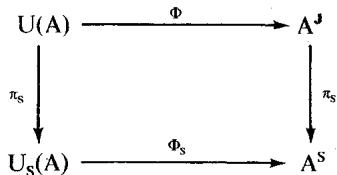
\includegraphics[keepaspectratio]{images/part001_3bc9714d.jpg}}

\(\mathrm{where}\ \Phi_{\mathbf{S}}((a_n)_{n\in \mathbf{S}}) = (\Phi_n((a_d)_{d\in \mathbf{J}_n}))_{n\in \mathbf{S}}.\)

\begin{enumerate}
\def\labelenumi{\alph{enumi})}
\setcounter{enumi}{1}
\item
  对每个 \(n \in \mathbf{J}\)，\(\operatorname{Ker}(\pi_{\mathrm{S}})\) 在 \(\mathbf{V}_{n}\) 下稳定，且 \(\operatorname{Ker}(\pi_{\mathrm{S}})\) 包含 \(\mathbf{V}_{n}(\mathrm{U}(\mathrm{A}))\)（若 \(n \notin S\)）。通过过渡到商，\(\mathbf{V}_{n}\) 定义了一个自同态，仍记作 \(\mathbf{V}_{n}\)，即 \(\mathrm{U}_{\mathrm{S}}(\mathrm{A})\) 的加法群的自同态。
\item
  若 \(n \in \mathbf{J}\) 且 \(n\mathbf{S} \subset \mathbf{S}\)，则 \(\operatorname{Ker}(\pi_{\mathbf{S}})\) 在 \(\mathbf{F}_{n}\) 下稳定，从而通过过渡到商定义了一个自同态，仍记作 \(\mathbf{F}_{n}\)，即环 \(\mathrm{U}_{\mathrm{S}}(\mathrm{A})\) 的自同态。
\end{enumerate}

\(d)\) 设 \(n \in \mathbf{J}\)。环 \(\mathrm{U}_{\mathrm{S}}(\mathrm{A})\) 也记作 \(\mathrm{U}_{n}(\mathrm{A})\)（若 \(S = \mathbf{J}_{n}\)），而记作 \(\mathrm{U}_{n\infty}(\mathrm{A})\)（若 \(\mathrm{S} = \bigcup_{n > 1} \mathbf{J}_{n}\)）。

设 \(p\) 是素数。证明 \(\mathrm{U}_{p^{\infty}}(\mathbf{A})\) 等同于维特环 \(\mathrm{W}(\mathbf{A})\)，且对每个 \(n \in \mathbf{N}\)，\(\mathrm{U}_{p^n}(\mathbf{A})\) 等同于环 \(\mathrm{W}_{n+1}(\mathbf{A})\)（我们把元素 ( \(u_1, u_p, u_{p^2}, ..., u_{p^{n-1}}, u_{p^n}\) )（\(\mathrm{U}_{p^n}(\mathbf{A})\) 的元素）等同于维特向量 \([a_0, ..., a_n]\)，其中 \(a_i = u_{p^i}\)（对 \(0 \leqslant i \leqslant n\)））。群自同态 \(\mathbf{V}_p\) 与 \(\mathbf{F}_p\)（\(\mathrm{U}_{p^\infty}(\mathbf{A})\) 的群自同态）在这一等同之下分别对应于 \(\mathrm{W}(\mathbf{A})\) 的位移与弗罗贝尼乌斯自同态。

\begin{enumerate}
\def\labelenumi{\arabic{enumi})}
\setcounter{enumi}{39}
\tightlist
\item
  设 A 是一个环。设 \(\mathbf{J} = \mathbf{P} \times \mathbf{Q}\) 是幺半群 J 分解为子幺半群 P 与 Q 之积的一个分解（于是它们由其所含的素数生成）。假设每个 \(q \in \mathbf{Q}\) 在 A 中可逆，从而在 U(A) 中也可逆（第 52 页，习题 35, e)）。a) 对每个 \(a \in \mathrm{U(A)}\)，级数
\end{enumerate}

\[
\varepsilon_ {\mathbf {Q}} (\boldsymbol {a}) = \sum_ {q \in \mathbf {Q}} \frac {\mu (q)}{q} \mathbf {V} _ {q} \mathbf {F} _ {q} (a),
\]

其中 \(\mu\) 表示默比乌斯函数（LIE, II, 第 71 页），对 U(A) = A \(^{J}\) 的乘积拓扑收敛。于是这就定义了 U(A) 的加法自同态 \(\varepsilon_{Q} = \sum_{q \in Q} \frac{\mu(q)}{q} V_{q} F_{q}\)。对每个 \(n \in J\)，映射 \(\Phi_{n} \circ \varepsilon_{Q}\)（从 U(A) 到 A 中的映射）等于 0（若 \(n \notin P\)），而等于 \(\Phi_{n}\)（若 \(n \in P\)）。b) 对每个 \(q \in Q\)（\(q \neq 1\)），有

\[
\varepsilon_ {\mathbf {Q}} \mathbf {V} _ {q} = 0 = \mathbf {F} _ {q} \varepsilon_ {\mathbf {Q}}.
\]

（利用 A, 第 52 页，习题 36, c)）。

\begin{enumerate}
\def\labelenumi{\alph{enumi})}
\setcounter{enumi}{2}
\tightlist
\item
  证明 \(\varepsilon_{\mathbf{Q}}\) 是一个幂等元，其像是诸 \(\mathbf{F}_{q}\)（\(q \in \mathbf{Q}, q \neq 1\)）的核的交。
\end{enumerate}

对 \(m \in \mathbf{J}\) 与 \(a \in \mathbf{A}\)，计算 \(\varepsilon_{\mathrm{Q}} \mathrm{V}_{m} \tau(a)\)。由此推出 \(\varepsilon_{\mathrm{Q}}\) 的核是形如 \(\sum_{n \in \mathrm{Q}} \mathrm{V}_{n} \tau(a_{n})\) 的元素（\(a_{n} \in \mathbf{A}\)）所成的集合。子集 \(\varepsilon_{\mathrm{Q}} \mathrm{U}(\mathrm{A})\)（\(\mathrm{U}(\mathrm{A})\) 的子集）在加法与乘法下稳定。赋以这两个运算后，它是一个交换环，单位元为 \(\varepsilon_{\mathrm{Q}}(1_{\mathrm{U}(\mathrm{A})})\)，且映射 \(\varepsilon_{\mathrm{Q}}: \mathrm{U}(\mathrm{A}) \to \varepsilon_{\mathrm{Q}} \mathrm{U}(\mathrm{A})\) 是环同态。

\begin{enumerate}
\def\labelenumi{\alph{enumi})}
\setcounter{enumi}{3}
\tightlist
\item
  对每个 \(q \in Q\)，令 \(e_{q} = \frac{1}{q} V_{q} \varepsilon_{Q} F_{q}\)。证明我们有 \(e_{q}^{2} = e_{q}\) 与 \(e_{q} e_{q'} = 0\)（当 \(q \neq q'\) 时），且对每个 \(a \in U(A)\)，我们有
\end{enumerate}

\[
(*) \quad \boldsymbol {a} = \sum_ {q \in Q} e _ {q} (\boldsymbol {a}),
\]

其中和式对 U(A) 的乘积拓扑收敛。（对于 (*)，化归到 \(a = X \in \mathrm{U}(\mathbf{R}[\mathbf{X}])\) 的情形，这里 R 是由分母属于 Q 的有理数所构成的 Q 的子环。这时只需应用 \(\Phi\)，并验证 (*) 在 \(\mathbf{R}[\mathbf{X}]^{\mathbf{J}}\) 中的类似式，它可由公式 \(\Phi_{pq} \circ e_{q'} = \Phi_{pq} \delta_{qq'}\)（若 \(p \in P\)，\(q \in Q\)，\(q' \in Q\)）得出。

子集 \(e_q \mathrm{U(A)}\)（\(\mathrm{U(A)}\) 的子集）在加法与乘法下稳定。赋以这两个运算后，它是一个交换环，单位元为 \(e_q(1_{\mathrm{U(A)}})\)，且映射 \(e_q: \mathrm{U(A)} \to e_q \mathrm{U(A)}\) 是环同态。

\begin{enumerate}
\def\labelenumi{\alph{enumi})}
\setcounter{enumi}{4}
\tightlist
\item
  对每个 \(q \in \mathbf{Q}\)，有 \(\mathbf{F}_q e_q = \varepsilon_{\mathbf{Q}} \mathbf{F}_q\) 与 \(\left(\frac{1}{q} \mathbf{V}_q\right) \varepsilon_{\mathbf{Q}} = e_q \left(\frac{1}{q} \mathbf{V}_q\right)\)。由此推出 \(\boldsymbol{a} \mapsto \mathbf{F}_q(\boldsymbol{a})\)
\end{enumerate}

是环同构 \(e_q\mathrm{U(A)}\to \varepsilon_{\mathrm{Q}}\mathrm{U(A)}\)，其逆为 \(\pmb {a}\mapsto \frac{1}{q}\mathbf{V}_q(\pmb {a})\)

\begin{enumerate}
\def\labelenumi{\alph{enumi})}
\setcounter{enumi}{5}
\item
  证明典范投影 \(\pi_{\mathbb{P}}: \mathrm{U}(\mathrm{A}) \to \mathrm{U}_{\mathbb{P}}(\mathrm{A})\)（习题 39）定义了环同构 \(\varepsilon_{\mathbb{Q}} \mathrm{U}(\mathrm{A}) \to \mathrm{U}_{\mathbb{P}}(\mathrm{A})\)。由此推出一个从 U(A) 到 \(\mathrm{U}_{\mathbb{P}}(\mathrm{A})^{\mathbb{Q}}\) 上的环同构，它把 \(a\) 映到 \((\pi_{\mathbb{P}} \varepsilon_{\mathbb{Q}} \mathrm{F}_{q}(a))_{q \in \mathbb{Q}}\)（对每个 \(a \in \mathrm{U}(\mathrm{A})\)）。
\item
  若 A 是一个 Q -代数，则可取 \(\mathbf{P} = \{1\}\) 与 \(\mathbf{Q} = \mathbf{J}\)。由此得到环同构 \(\mathrm{U}(\mathrm{A}) \to \mathrm{A}^{\mathbf{J}}\)，它不是别的，正是 \(\Phi\)。
\end{enumerate}

  \(h)\) 设 \(\mathbf{P} = \{p^n | n \in \mathbb{N}\}\)，其中 \(p\) 是素数。于是每个素数 \(q \neq p\) 都在 A 中可逆。我们得到一个环同构 \(\mathrm{U(A)} \to \mathrm{W(A)}^{\mathrm{Q}}\)（参见习题 39, \(d\)））。

我们以 \(\omega_{\mathrm{A}}\) 表示从 W(A) 到 U(A) 中的映射，它经由 U(A) 与 \(\mathrm{W(A)}^{\mathbf{Q}}\) 之间的同构，对应于 W(A) 按第一个分量在 \(\mathrm{W(A)}^{\mathbf{Q}}\) 中的嵌入。

\begin{enumerate}
\def\labelenumi{\arabic{enumi})}
\setcounter{enumi}{40}
\tightlist
\item
  设 A 是一个环。
\end{enumerate}

\begin{enumerate}
\def\labelenumi{\alph{enumi})}
\tightlist
\item
  设 \(\mu: A \to U(A)\) 是环同态，满足 \(\Phi_1 \circ \mu = \text{Id}_A\)。令 \(\sigma = \Phi \circ \mu\) 且 \(\sigma(a) = (\sigma_n(a))_{n \in J}\)（对 \(a \in A\)）。诸映射 \(\sigma_n: A \to A (n \in J)\) 满足下列条件：
\end{enumerate}

\begin{enumerate}
\def\labelenumi{(\arabic{enumi})}
\item
  \(\sigma_{n}\) 是环同态（对每个 \(n\in\mathbf{J}\)），且 \(\sigma_{1}=\mathrm{Id}_{\mathbf{A}}\)。
\item
  对每个素数 \(p\) 与所有 \(a \in \mathbf{A}\)，有 \(\sigma_p(a) \equiv a^p \mod p\mathbf{A}\) and
\end{enumerate}

\[
\sigma_ {p} \left(\sigma_ {n} (a)\right) \equiv \sigma_ {p n} (a) \bmod . p ^ {w _ {p} (p n)} \mathrm{A} \quad \text { for every } \quad n \in \mathbf {J}.
\]

\begin{enumerate}
\def\labelenumi{\alph{enumi})}
\setcounter{enumi}{1}
\item
  设 A 的加法群在 Z 上无挠。设 \(\sigma = (\sigma_n)_{n \in \mathbf{J}}\) 是一族映射 \(\sigma_n: A \to A\)，满足 \(a\)）中的条件 (1) 与 (2)。存在唯一的环同态 \(\mu: A \to U(A)\)，使得 \(\Phi_1 \circ \mu = Id_A\) 且 \(\Phi \circ \mu = \sigma\)（应用 A, 第 51 页，习题 32 与 33, \(d\)）。）
\item
  设 A 的加法群在 Z 上无挠。存在唯一的环同态
\end{enumerate}

\[
\mu^ {\mathrm{A}}: \mathrm{U} (\mathrm{A}) \rightarrow \mathrm{U} (\mathrm{U} (\mathrm{A}))
\]

使得 \(\Phi^{\mathrm{U(A)}}\circ \mu^{\mathrm{A}}\) 是映射

\[
\mathbf {F} ^ {\mathbf {A}}: \mathrm{U} (\mathbf {A}) \rightarrow \mathrm{U} (\mathbf {A}) ^ {\mathbf {J}}
\]

它由 \(\mathbf{F}^{\mathrm{A}}(\boldsymbol{a}) = (\mathbf{F}_n(\boldsymbol{a}))_{n\in \mathbf{J}}\) 定义（化归到 \(\mathbf{A} = \mathbf{Z}[\mathbf{X}]\) 的情形，并应用 \(b\)）以及 A, 第 52 页习题 36 与 A, 第 53 页习题 38, \(b\)）。）

\begin{enumerate}
\def\labelenumi{\alph{enumi})}
\setcounter{enumi}{3}
\tightlist
\item
  设 \(\mathbf{X} = (\mathbf{X}_n)_{n\in \mathbf{J}}\) 是一个未定元族，视为 \(\mathrm{U}(\mathbf{Z}[\mathbf{X}])\) 的一个元素。令
\end{enumerate}

\[
\mu^ {\mathbf {Z} [ \mathbf {X} ]} (\mathbf {X}) = \left(\mu_ {n} (\mathbf {X})\right) _ {n \in \mathbf {J}} = \left(\left(\mu_ {n, m} (\mathbf {X})\right) _ {m \in \mathbf {J}}\right) _ {n \in \mathbf {J}}
\]

其中 \(\mu_{n,m}(\mathbf{X})\in\mathbf{Z}[\mathbf{X}]\)（对 \(n,m\in\mathbf{J}\)）。对每个环 A，定义 \(\mu^{\mathbf{A}}:\mathrm{U}(\mathbf{A})\to\mathrm{U}(\mathrm{U}(\mathbf{A}))\)：\(\mu^{\mathbf{A}}(\boldsymbol{a})=(\left(\mu_{n,m}(\boldsymbol{a})\right)_{m\in\mathbf{J}})_{n\in\mathbf{J}}\)。证明 \(\mu^{\mathbf{A}}\) 是环同态，且使下列图交换

\begin{enumerate}
\def\labelenumi{(\arabic{enumi})}
\tightlist
\item
\end{enumerate}

\pandocbounded{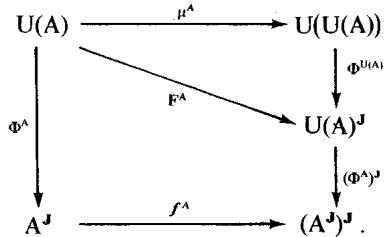
\includegraphics[keepaspectratio]{images/part001_e852df9c.jpg}}

这里按定义，\(f^{\mathrm{A}}(\boldsymbol{a}) = (f_n(\boldsymbol{a}))_{n \in \mathbf{J}}\)（对 \(\boldsymbol{a} \in \mathrm{A}^{\mathrm{J}}\)），而 \(\Phi^{\mathrm{A}}\)（相应地，\(\Phi^{\mathrm{U(A)}}\)）是与环 A（相应地，U(A)）相伴的同态 \(\Phi\)。

\begin{enumerate}
\def\labelenumi{\alph{enumi})}
\setcounter{enumi}{4}
\tightlist
\item
  对每个环同态 \(\rho: \mathbf{B} \to \mathbf{A}\)，图
\end{enumerate}

\pandocbounded{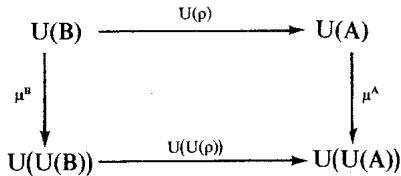
\includegraphics[keepaspectratio]{images/part001_6be88655.jpg}}

是交换的。

\begin{enumerate}
\def\labelenumi{\alph{enumi})}
\setcounter{enumi}{5}
\tightlist
\item
  证明下列图是交换的。
\end{enumerate}

\pandocbounded{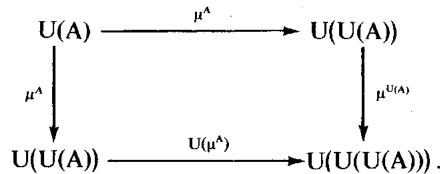
\includegraphics[keepaspectratio]{images/part001_4b4fe1b3.jpg}}

（化归到 A = \(\mathbf{Q}[\mathbf{X}]\) 的情形。这时 A 是一个 Q -代数，因而 \(\Phi^{\mathbf{A}}: \mathrm{U}(\mathrm{A}) \to \mathrm{A}^{\mathbf{J}}\) 是同构，且 U(A) 也是一个 Q -代数。若当 A 是 Q -代数时，利用图 (1) 并通过结构的转移把 \(\mu^{\mathbf{A}}\) 换成 \(f^{\mathbf{A}}\)，则问题化为证明图的交换性

\pandocbounded{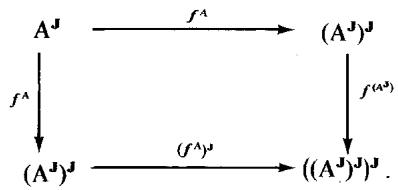
\includegraphics[keepaspectratio]{images/part001_85799ba9.jpg}}

我们有

\[
f ^ {(\mathrm{A} ^ {\mathrm{J}})} \left(f ^ {\mathrm{A}} (\mathbf {X})\right) = f ^ {(\mathrm{A} ^ {\mathrm{J}})} \left(\left(f _ {n} (\mathbf {X})\right) _ {n \in \mathbf {J}}\right) = \left(\left(f _ {m} \left(f _ {n} (\mathbf {X})\right)\right) _ {n \in \mathbf {J}}\right) _ {m \in \mathbf {J}} = \left(\left(f _ {m n} (\mathbf {X})\right) _ {n \in \mathbf {J}}\right) _ {m \in \mathbf {J}},
\]

以及

\[
(f ^ {\mathrm{A}}) ^ {\mathrm{J}} (f ^ {\mathrm{A}} (\mathbf {X})) = (f ^ {\mathrm{A}}) ^ {\mathrm{J}} ((f _ {n} (\mathbf {X})) _ {n \in \mathbf {J}}) = (f ^ {\mathrm{A}} (f _ {n} (\mathbf {X}))) _ {n \in \mathbf {J}} = ((f _ {m n} (\mathbf {X})) _ {m \in \mathbf {J}}) _ {n \in \mathbf {J}}.
\]

\begin{enumerate}
\def\labelenumi{\alph{enumi})}
\setcounter{enumi}{6}
\tightlist
\item
  对每个 \(a \in \mathbf{A}\)，有
\end{enumerate}

\[
\mu_ {n} ^ {\mathrm{A}} (\tau (a)) = 0 \quad \text { for } \quad n \geqslant 2.
\]

\begin{enumerate}
\def\labelenumi{\alph{enumi})}
\setcounter{enumi}{7}
\tightlist
\item
  我们有下列交换图
\end{enumerate}

\pandocbounded{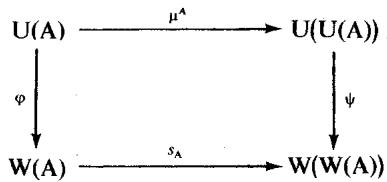
\includegraphics[keepaspectratio]{images/part001_0d6c50d0.jpg}}

其中映射 \(s_{\mathbf{A}}\) 是 A, 第 44 页，习题 15 中定义的映射，映射 \(\varphi\)（从 U(A) 到 W(A) 中的映射）是通过把 W(A) 与 U \(_{p\infty}\) (A) 等同（第 53 页，习题 39）而得到的，而映射 \(\psi\) 是 U( \(\varphi\) ) 与从 U(W(A)) 到 W(W(A)) 中的映射（通过把 W(W(A)) 与 U \(_{p\infty}\) (W(A)) 等同而得到）的复合。

\begin{enumerate}
\def\labelenumi{\arabic{enumi})}
\setcounter{enumi}{41}
\tightlist
\item
  设 A 是一个环，T 是未定元。我们以 \(\Lambda(A)\)（或 \(\Lambda_{T}(A)\)）表示 \(1 + TA[[T]]\)，即系数在 A 中且常数项等于 1 的形式幂级数所成的集合；它是 \(A[[T]]\) 的乘法群的一个子群。我们定义
\end{enumerate}

\[
\mathrm{L}: \Lambda (\mathrm{A}) \rightarrow \mathrm{A} ^ {\mathbf {J}}, \quad \mathrm{L} (f) = \left(\mathrm{L} _ {n} (f)\right) _ {n \in \mathbf {J}},
\]

为

\[
- \mathrm{T} \frac {d f}{d \mathrm{T}} / f = \sum_ {n \in \mathbf {J}} \mathrm{L} _ {n} (f) (- \mathrm{T}) ^ {n}.
\]

\begin{enumerate}
\def\labelenumi{\alph{enumi})}
\item
  证明对任意的 f, g ∈ Λ(A)，有 L(fg) = L(f) + L(g)。
\item
  若 A 是一个 Q -代数，则 L 是双射，其逆 ε 由下式给出
\end{enumerate}

\[
\varepsilon (\boldsymbol {a}) = \exp (- \sum_ {n \in \mathbf {J}} \frac {a _ {n}}{n} (- \mathrm{T}) ^ {n})
\]

（对 \(a \in A^{J}\)）。

\begin{enumerate}
\def\labelenumi{\arabic{enumi})}
\setcounter{enumi}{42}
\tightlist
\item
  设 E: U(A) → Λ(A) 是由下式定义的映射
\end{enumerate}

\[
\mathrm{E} (\boldsymbol {a}) = \prod_ {n \in \mathbf {J}} (1 - a _ {n} (- \mathrm{T}) ^ {n})
\]

（对 \(a \in \mathrm{U}(\mathrm{A})\)）。

\begin{enumerate}
\def\labelenumi{\alph{enumi})}
\tightlist
\item
  证明图的交换性。
\end{enumerate}

\pandocbounded{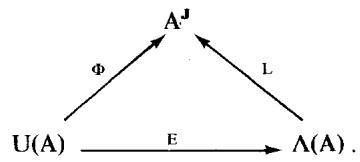
\includegraphics[keepaspectratio]{images/part001_4add4456.jpg}}

由此推出，若 A 是一个 Q -代数，则

\[
\prod_ {n \in \mathbf {J}} (1 - a _ {n} \mathrm{T} ^ {n}) = \exp \left(- \sum_ {n \in \mathbf {J}} (\Phi_ {n} (\boldsymbol {a}) / n) \mathrm{T} ^ {n}\right)
\]

（对每个 \(a \in \mathrm{U}(\mathrm{A})\)）。

\begin{enumerate}
\def\labelenumi{\alph{enumi})}
\setcounter{enumi}{1}
\item
  证明 E 是双射。（若令 \(\prod_{n\in J}(1 - a_n(-T)^n) = \sum_{n\geqslant 0}c_n(a)(-T)^n\)，则只需对多项式族 \(c_{n}(\mathbf{X})\)（\(\mathbf{Z}[\mathbf{X}]\) 中的多项式）应用 A, 第 51 页，习题 33, a)。）
\item
  我们给 \(\Lambda(A)\) 赋以使 E 成为环同构的唯一环结构。证明 \(\Lambda(A)\) 的加法就是级数的乘法，其单位元为 1。环 \(\Lambda(A)\) 的乘法记作 \((f,g)\mapsto f*g\)，由下列公式定义
\end{enumerate}

\[
\mathrm{E} (\boldsymbol {a} \times \boldsymbol {b}) = \mathrm{E} (\boldsymbol {a}) * \mathrm{E} (\boldsymbol {b})
\]

（对任意的 \(a, b \in \mathrm{U}(\mathrm{A})\)）；它的单位元是 \(1 + T\)。

\begin{enumerate}
\def\labelenumi{\alph{enumi})}
\setcounter{enumi}{3}
\tightlist
\item
  设 \(\tau : \mathrm{A} \to \mathrm{U}(\mathrm{A})\) 是 A, 第 53 页，习题 37, c) 中定义的映射。我们有
\end{enumerate}

\[
\begin{array}{c} \mathrm{E} (\tau (a)) = 1 + a \mathrm{T} \\ (1 + a \mathrm{T}) * (1 + b \mathrm{T}) = 1 + a b \mathrm{T} \\ (1 + a \mathrm{T}) * f (\mathrm{T}) = f (a \mathrm{T}) \\ \mathrm{L} (1 + a \mathrm{T}) = (a ^ {n}) _ {n \in \mathbf {J}} \end{array}
\]

（对任意 \(a, b\)（在 \(\mathbf{A}\) 中）与 \(f(\mathbf{T})\)（在 \(\Lambda(\mathbf{A})\) 中））。

\begin{enumerate}
\def\labelenumi{\alph{enumi})}
\setcounter{enumi}{4}
\tightlist
\item
  设 \(f\) 与 \(g\) 是 \(\Lambda(A)\) 的两个元素，它们都是 \(T\) 的多项式，并设 \(m\) 为 \(f\) 的次数。令
\end{enumerate}

\[
\varphi (\mathrm{X}) = \mathrm{X} ^ {m} f (\mathrm{T} / \mathrm{X})
\]

以及

\[
\gamma (\mathrm{X}) = g (- \mathrm{X}).
\]

它们是系数在 A\([\mathrm{T}]\) 中的 X 的多项式；\(\varphi\) 是首一的，且 \(f*g\) 是结式 \(\operatorname{res}(\varphi, \gamma)\)——多项式 \(\varphi\) 与 \(\gamma\) 的结式（参见 A, IV, 第 75 页）。

（可以从公式

\[
(1 + a \mathrm{T}) * g = g (a \mathrm{T}),
\]

出发，对 \(A = \mathbf{Z}[X_{1}, \ldots, X_{m}]\) 且 \(f = \prod_{i=1}^{m} (1 + X_i \mathrm{T})\) 的情形推出结果，再从那里过渡到一般情形。）

\begin{enumerate}
\def\labelenumi{\arabic{enumi})}
\setcounter{enumi}{43}
\tightlist
\item
  设 A 是一个环。
\end{enumerate}

\begin{enumerate}
\def\labelenumi{\alph{enumi})}
\item
  集合 \(\hat{\mathbf{U}}(\mathbf{A})\)——由 \(\mathrm{U}(\mathbf{A})\) 中坐标为幂零且除有限多个外皆为零的元素组成——是环 \(\mathrm{U}(\mathbf{A})\) 的一个理想。对每个 \(n \in \mathbf{J}\)，它在 \(\mathrm{F}_n\) 与 \(\mathrm{V}_n\) 下稳定。
\item
  设 \(\boldsymbol{a} \in \hat{\mathbf{U}}(\mathbf{A})\)。则元素 \(\mathrm{E}(\boldsymbol{a})\)（\(\Lambda(\mathbf{A})\) 中的元素）是 T 的一个多项式。它在 \(-1\) 处的值是 A 的一个可逆元；对每个 \(n \in \mathbf{J}\)，它也是 \(-1\) 处多项式 \(\mathrm{E}(\mathrm{V}_n\boldsymbol{a})\) 的值。
\item
  若 \(\boldsymbol{a} \in \mathrm{U}(\mathbf{A})\) 且 \(\boldsymbol{b} \in \hat{\mathbf{U}}(\mathbf{A})\)，以 \(\langle \boldsymbol{a}, \boldsymbol{b} \rangle\) 表示 \(-1\) 处多项式 \(\mathrm{E}(\boldsymbol{a}\boldsymbol{b})\) 的值。这样就定义了一个从 \(\mathrm{U}(\mathbf{A}) \times \hat{\mathbf{U}}(\mathbf{A})\) 到 \(\mathbf{A}^*\) 中的 Z -双线性映射，且有
\end{enumerate}

\[
\begin{array}{l} \langle \mathbf {F} _ {n} \boldsymbol {a}, \boldsymbol {b} \rangle = \langle \boldsymbol {a}, \mathbf {V} _ {n} \boldsymbol {b} \rangle \\ \langle \mathbf {V} _ {n} \boldsymbol {a}, \boldsymbol {b} \rangle = \langle \boldsymbol {a}, \mathbf {F} _ {n} \boldsymbol {b} \rangle \quad \text { for every } n \in \mathbf {J}. \end{array}
\]

\begin{enumerate}
\def\labelenumi{\arabic{enumi})}
\setcounter{enumi}{44}
\tightlist
\item
  所谓预 λ -环，是指一个环 A，带有一族映射 \(\lambda_{n}: \mathbf{A} \to \mathbf{A} (n \in \mathbb{N})\)，使得 (i) \(\lambda_{0}(a) = 1\)，
\end{enumerate}

\begin{enumerate}
\def\labelenumi{(\roman{enumi})}
\setcounter{enumi}{1}
\item
  \(\lambda_{1}(a) = a,\)
\item
  \(\lambda_{n}(a + b) = \sum_{p=0}^{n} \lambda_{p}(a) \lambda_{n-p}(b)\) ,
\end{enumerate}

对 A 中任意的 \(a, b\)。条件 (i) 与 (iii) 也可以表述为

\[
\lambda (a) = \sum_ {n \geqslant 0} \lambda_ {n} (a) \mathrm{T} ^ {n}
\]

定义了一个从 A 的加法群到乘法群 \(\Lambda(A)\) 中的同态。

所谓预 \(\lambda\) -环 A 到另一个预 λ -环 B 中的 \(\lambda\) -态射，是指一个环同态 \(\rho: A \to B\)，使得 \(\rho(\lambda_n(a)) = \lambda_n(\rho(a))\)（对任意的 \(a \in A\)，\(n \in \mathbf{N}\)），换言之，使得图

\pandocbounded{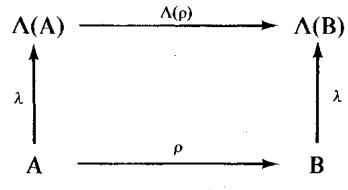
\includegraphics[keepaspectratio]{images/part001_12576e27.jpg}}

是交换的（映射 \(\Lambda(\rho)\) 把级数 \(1 + \sum_{n\geqslant 1}a_n\mathrm{T}^n\) 变为级数 \(1 + \sum_{n\geqslant 1}\rho(a_n)\mathrm{T}^n\)）。设 A 是一个环。我们打算给 \(\Lambda(\mathbf{A})\) 赋以一个预 \(\lambda\) -环结构。我们以 \(\mathbf{E}^{\mathbf{A}}:\mathrm{U}(\mathbf{A})\to \Lambda_{\mathbf{T}}(\mathbf{A})\) 表示习题 43 中定义的环同构。设 S 是另一个未定元。

\begin{enumerate}
\def\labelenumi{\alph{enumi})}
\tightlist
\item
  证明两个复合同构
\end{enumerate}

\[
\mathrm{U} (\mathrm{U} (\mathrm{A})) \xrightarrow {\mathrm{U} (\mathrm{E} ^ {\mathrm{A}})} \mathrm{U} (\Lambda_ {\mathrm{T}} (\mathrm{A})) \xrightarrow {\mathrm{E} ^ {\Lambda_ {\mathrm{T}} (\mathrm{A})}} \Lambda_ {\mathrm{S}} (\Lambda_ {\mathrm{T}} (\mathrm{A}))
\]

以及

\[
\mathrm{U} (\mathrm{U} (\mathrm{A})) \xrightarrow {\mathrm{E} ^ {\mathrm{U} (\mathrm{A})}} \Lambda_ {\mathrm{S}} (\mathrm{U} (\mathrm{A})) \xrightarrow {\Lambda_ {\mathrm{S}} (\mathrm{E} ^ {\mathrm{A}})} \Lambda_ {\mathrm{S}} (\Lambda_ {\mathrm{T}} (\mathrm{A}))
\]

相重合；我们将把它们记作 \(\tilde{\mathbf{E}}^{\mathbf{A}}\)。

我们用图的交换性来定义映射 \(\lambda^{\mathrm{A}}\)

\pandocbounded{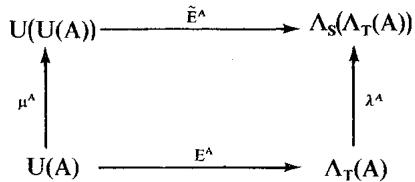
\includegraphics[keepaspectratio]{images/part001_a93606d8.jpg}}

其中 \(\mu^{\mathbf{A}}\) 表示 A, 第 55 页，习题 41, \(d\)）中定义的同态。

\begin{enumerate}
\def\labelenumi{\alph{enumi})}
\setcounter{enumi}{1}
\item
  环 \(\Lambda(A)\)，赋以 \(\lambda^{A}\) 后，是一个预 \(\lambda\) -环。对每个环同态 \(\rho: A \to B\)，\(\Lambda(\rho): \Lambda(A) \to \Lambda(B)\) 是一个 \(\lambda\) -态射。
\item
  预 λ -环 A 称为 λ -环，如果 λ: A → Λ(A) 是一个 λ -态射（对刚才定义的 Λ(A) 上的预 λ -环结构而言）。
\end{enumerate}

设 A 是一个环。证明 \((\Lambda(A), \lambda^A)\) 是一个 \(\lambda\) -环。（利用 A, 第 56 页，习题 41, \(f\)）。）

\begin{enumerate}
\def\labelenumi{\arabic{enumi})}
\setcounter{enumi}{45}
\tightlist
\item
  \begin{enumerate}
  \def\labelenumii{\alph{enumii})}
  \tightlist
  \item
    设 A 是一个预 λ -环，\(a \in A\)。a 的 λ -秩称为 \(\overline{R}\) 中整数 \(n \in N\)（使得 \(\lambda_{n}(a) \neq 0\)）所成集合的上确界。设 P 是 A 的一个由 λ -秩 \(\leqslant 1\) 的元素组成的乘法子集。设 \(a = \sum_{i \in I} a_{i}\) 是 P 的元素的一个有限族之和。我们有 \(\lambda(a) = \prod_{i \in I} (1 + a_i T)\)，从而 \(\lambda_n(a) = s_n((a_i)_{i \in I})\)，其中 \(s_n\) 表示初等对称多项式
  \end{enumerate}
\end{enumerate}

其次数为 n（A, IV, 第 63 页）。

\begin{enumerate}
\def\labelenumi{\alph{enumi})}
\setcounter{enumi}{1}
\item
  设 A 是一个环，\(a, b\) 是 A 的元素。则在 \(\Lambda(A)\) 中，元素 \(1 + aT\) 与 \((1 + aT)*(1 + bT) = 1 + abT\) 的 \(\lambda\) -秩都 \(\leqslant 1\)。
\item
  设 A 是一个预 λ -环。假设存在 A 的一个乘法子幺半群，由 λ -秩 ≤ 1 的元素组成，它生成 A 的加法群。证明这时 A 是一个 λ -环。更一般地，若存在一个从 A 到满足前述性质的预 λ -环中的单射 λ -态射，则 A 是 λ -环（“分裂原理”）。（问题在于证明 Z -双线性映射 \((a, b) \mapsto \lambda(a) * \lambda(b) * \lambda(ab)^{-1}\) 为零，并且证明 Z -线性映射 \(a \mapsto \Lambda_{\mathrm{S}}(\lambda_{\mathrm{T}})[\lambda_{\mathrm{S}}(a)]\) 与 \(a \mapsto \lambda_{\mathrm{S}}^{\mathrm{A}}(\lambda_{\mathrm{T}}(a))\)（都是从 A 到 \(\Lambda_{\mathrm{S}}(\Lambda_{\mathrm{T}}(\mathrm{A}))\) 中的映射）相重合。只需对 \(a, b \in P\) 验证这些性质即可。）
\item
  设 \(A = \mathbf{Z}[(X_i)_{i\in I}, (X_{i'}')_{i'\in I'}]\) 是两个有限未定元族的多项式环。我们有
\end{enumerate}

\[
\prod_ {i \in I} (1 + X _ {i} T) = \sum_ {n \geqslant 0} s _ {n} ((X _ {i}) _ {i \in I}) T ^ {n}
\]

其中

\[
s _ {n} \left(\left(X _ {i}\right) _ {i \in I}\right) = \sum_ {\mathrm{H} \in \binom {I} {n}} X _ {\mathrm{H}},
\]

其中 \(\binom{I}{n}\) 表示 I 的具有 n 个元素的子集所成的集合，而 \(X_{H} = \prod_{h \in H} X_{h}\)。给 \(X_{i}\)（以及 \(X_{i'}\)）赋以权 1，则 \(s_{n}\) 是权 n 的齐次多项式。\((X_{i})_{i \in I}\) 的每个对称多项式都可以唯一地表示为 \(s_{n}\)（\(n \geqslant 1\)）的多项式（A, IV, 第 58 页）。特别地，对每个 \(m \geqslant 0\)，有

\[
s _ {m} \left(\left(\mathrm{X} _ {\mathrm{H}}\right) _ {\mathrm{H} \in \binom {\mathrm{I}} {n}}\right) = \mathrm{Q} _ {n, m} \left(s _ {1}, \dots , s _ {n m}\right)
\]

其中 \(Q_{n,m}\) 关于诸 \(s_r = s_r((X_i)_{i \in I}) (r = 1, \ldots, nm)\) 是权 nm 的齐次多项式。它是 \(T^m\) 在 \(\prod (1 + X_H T)\) 中的系数，只要 \(\text{Card}(I) \geqslant nm\)，它就有良好的定义且与 I 无关。

\(\mathbf{T}^n\) 在 \(\prod (1 + X_iX_i'T)\) 中的系数是

\[
s _ {n} \left(\left(X _ {i} X _ {i ^ {\prime}} ^ {\prime}\right) _ {(i, i ^ {\prime}) \in I \times I ^ {\prime}}\right) = P _ {n} \left(s _ {1}, \dots , s _ {n}, s _ {1} ^ {\prime}, \dots , s _ {n} ^ {\prime}\right)
\]

其中 \(s_r' = s_r((X_{i'}')_{i'\in I'})\)，而 \(P_n\) 是权 \(n\) 的齐次多项式——关于变量族 \((s_r)\) 与 \((s_r')\) 的每一个。只要 I 与 I' 的基数都 \(\geqslant n\)，它就有良好的定义且与 I 和 I' 无关。

证明在 \(\lambda\) -环 \(\Lambda(A)\) 中，我们有

\[
\left(\sum_ {r \geqslant 0} s _ {r} \mathrm{T} ^ {r}\right) * \left(\sum_ {r \geqslant 0} s _ {r} ^ {\prime} \mathrm{T} ^ {r}\right) = \sum_ {n \geqslant 0} \mathrm{P} _ {n} (s _ {1},..., s _ {n}, s _ {1} ^ {\prime},..., s _ {n} ^ {\prime}) \mathrm{T} ^ {n}
\]

以及

\[
\lambda_ {n} ^ {\mathrm{A}} \left(\sum_ {r \geqslant 0} s _ {r} \mathrm{T} ^ {r}\right) = \sum_ {m \geqslant 0} \mathrm{Q} _ {n, m} \left(s _ {1}, \dots , s _ {n m}\right) \mathrm{T} ^ {m}.
\]

由 a) 与 b)，我们有

\[
\left(\sum_ {r} s _ {r} \mathrm{T} ^ {r}\right) * \left(\sum_ {r} s _ {r} ^ {\prime} \mathrm{T} ^ {r}\right) = \left(\prod_ {i} \left(1 + \mathrm{X} _ {i} \mathrm{T}\right)\right) * \left(\prod_ {i ^ {\prime}} \left(1 + \mathrm{X} _ {i} ^ {\prime} \mathrm{T}\right)\right) = \prod_ {i, i ^ {\prime}} \left(1 + \mathrm{X} _ {i} \mathrm{X} _ {i ^ {\prime}} ^ {\prime} \mathrm{T}\right)
\]

以及

\[
\begin{array}{l} \lambda (\sum_ {r} s _ {r} \mathrm{T} ^ {r}) = \lambda (\prod _{i} (1 + X _ {i} \mathrm{T})) = \prod _{i} (1 + (1 + X _ {i} \mathrm{T}) \mathrm{S}) = \sum _{n} s _ {n} ((1 + X _ {i} \mathrm{T}) _ {i \in \mathrm{I}}) \mathrm{S} ^ {n} \\ \text{且}\quad s _ {n} ((1 + X _ {i} \mathrm{T}) _ {i \in \mathrm{I}}) = \prod _{\mathrm{H} \in \binom {\mathrm{I}} {n}} (1 + X _{\mathrm{H}} \mathrm{T}) . \end{array}
\]

\begin{enumerate}
\def\labelenumi{\alph{enumi})}
\setcounter{enumi}{4}
\tightlist
\item
  设 A 是一个预 λ -环。为使 A 是一个 λ -环，必要且充分的是下列条件对 A 中所有的 a, b 以及 N 中所有的 n, m 都成立。
\end{enumerate}

\begin{enumerate}
\def\labelenumi{(\roman{enumi})}
\item
  \(\lambda(1) = 1 + T,\)
\item
  \(\lambda_{n}(ab) = \mathrm{P}_{n}(\lambda_{1}(a),\dots,\lambda_{n}(a),\lambda_{1}(b),\dots,\lambda_{n}(b)),\)
\item
  \(\lambda_{m}(\lambda_{n}(a)) = Q_{n,m}(\lambda_{1}(a),\dots,\lambda_{nm}(a)).\)
\end{enumerate}

\begin{enumerate}
\def\labelenumi{\alph{enumi})}
\setcounter{enumi}{5}
\tightlist
\item
  设 \(\rho: A \to B\) 是预 \(\lambda\) -环的一个 \(\lambda\) -态射。若 A 是 \(\lambda\) -环且 \(\rho\) 是满射，则 B 是 \(\lambda\) -环。若 B 是 \(\lambda\) -环且 \(\rho\) 是单射，则 A 是 \(\lambda\) -环。
\end{enumerate}

\begin{enumerate}
\def\labelenumi{\arabic{enumi})}
\setcounter{enumi}{46}
\tightlist
\item
  设 A 是一个环。我们用下列公式定义映射 \(F_{n}\)、\(V_{n}\)（\(n \in \mathbf{J}\)），它们把 \(\Lambda(\mathbf{A})\) 映到其自身
\end{enumerate}

\[
\mathrm{F} _ {n} (\mathrm{E} (a)) = \mathrm{E} \left(\mathrm{F} _ {n} (a)\right), \quad \mathrm{V} _ {n} (\mathrm{E} (a)) = \mathrm{E} \left(\mathrm{V} _ {n} (a)\right)
\]

对所有 \(\boldsymbol{a} \in \mathrm{U}(\mathbf{A})\)。

\begin{enumerate}
\def\labelenumi{\alph{enumi})}
\tightlist
\item
  我们有 \(\mathrm{L}(\mathrm{F}_n(f)) = f_n(\mathrm{L}(f))\) 与 \(\mathrm{L}(\mathrm{V}_n(f)) = v_n(\mathrm{L}(f))\)，对所有 \(f \in \Lambda(\mathbf{A})\)。
\end{enumerate}

设 n, m 属于 J，并令 \(d = \operatorname{pgcd}(n, m)\)。

\begin{enumerate}
\def\labelenumi{\alph{enumi})}
\setcounter{enumi}{1}
\item
  证明 \(F_{n}\) 是环 \(\Lambda(\mathbf{A})\) 的一个自同态，并且我们有 \(F_{n} \circ F_{m} = F_{nm}\)。对每个素数 p 以及每个 \(f \in \Lambda(\mathbf{A})\)，有 \(F_{p}(f) \equiv f^{*p} \mod p * \Lambda(\mathbf{A})\)，其中 \(f^{*p}\) 表示环 \(\Lambda(\mathbf{A})\) 中 p 个都等于 f 的项之积，而 \(p * \Lambda(\mathbf{A})\) 表示 \(\Lambda(\mathbf{A})\) 的主理想，它由 \(\Lambda(\mathbf{A})\) 中 p 个都等于中性元 1 + T 的项之和（换言之，由 \((1 + T)^{p}\)）生成。
\item
  证明 \(V_{n}\) 是 \(\Lambda(\mathbf{A})\) 的加法群的一个自同态，并且我们有 \(V_{n} \circ V_{m} = V_{nm}\)。d) 对每个 \(f \in \Lambda(\mathbf{A})\)，有 \(F_{n}(V_{m}(f)) = V_{m/d}(F_{n/d}(f))^{d}\)。特别地 \(F_{n}(V_{n}(f)) = f^{n}\)，且 \(F_{n} \circ V_{m} = V_{m} \circ F_{n}\)（当 \(d = 1\) 时）。对任意 \(f,g\in\Lambda(\mathbf{A})\)，我们有
\item
  设 \(f, g\) 是 \(\Lambda(A)\) 中的任意元素，则有
\end{enumerate}

\[
\begin{array}{l} \mathrm{V} _ {n} (f) * \mathrm{V} _ {m} (g) = \mathrm{V} _ {n m / d} (\mathrm{F} _ {m / d} (f) * \mathrm{F} _ {n / d} (g)) ^ {d}, \\ \mathrm{V} _ {n} (f * \mathrm{F} _ {m} (g)) ^ {n / d} = \mathrm{V} _ {n} (f) * \mathrm{V} _ {n / d} (\mathrm{F} _ {m / d} (g)), \\ \mathrm{V} _ {n} (\mathrm{F} _ {m} (g)) ^ {n / d} = \mathrm{V} _ {n} (1 + \mathrm{T}) * \mathrm{V} _ {n / d} (\mathrm{F} _ {m / d} (g)). \end{array}
\]

特别地，我们有

以及

\[
\begin{array}{r l} & {\mathrm{V} _ {n} (f) * \mathrm{V} _ {n} (g) = \mathrm{V} _ {n} (f * g) ^ {n}} \\ & {\mathrm{V} _ {n} (f) * \mathrm{V} _ {m} (g) = \mathrm{V} _ {n m} (\mathrm{F} _ {m} (f) * \mathrm{F} _ {n} (g)) \quad \text {if} \quad d = 1.} \end{array}
\]

\begin{enumerate}
\def\labelenumi{\alph{enumi})}
\setcounter{enumi}{5}
\tightlist
\item
  我们有
\end{enumerate}

\[
\mathrm{V} _ {n} (f) (\mathrm{T}) = f (- (- \mathrm{T}) ^ {n})
\]

对所有 \(f \in \Lambda(\mathbf{A})\)。特别地

\[
\mathrm{V} _ {n} (1 + a \mathrm{T}) = 1 - a (- \mathrm{T}) ^ {n}
\]

对每个 \(a \in \mathbf{A}\)。

\begin{enumerate}
\def\labelenumi{\alph{enumi})}
\setcounter{enumi}{6}
\tightlist
\item
  对每个 \(a \in \mathbf{A}\)，有
\end{enumerate}

\[
\mathrm{F} _ {n} (1 + a \mathrm{T}) = 1 + a ^ {n} \mathrm{T}.
\]

对每个 \(f \in \Lambda(\mathbf{A})\)，有

\[
\mathrm{F} _ {n} (f) \left(- (- \mathrm{T}) ^ {n}\right) = \mathrm{N} (f (\mathrm{T}))
\]

其中 N 表示扩张 \(A[[\mathrm{T}^{n}]] \subset A[[\mathrm{T}]]\) 中的范数。（只需处理 \(f \in A[\mathrm{T}]\) 的情形，然后把 A 嵌入一个环 B，使 f 在其中分解成线性因子的乘积，再对之应用第一个公式即可。）

对每个 \(a \in \mathbf{A}\)，有

\[
\mathrm{F} _ {n} (1 - a (- \mathrm{T}) ^ {m}) = (1 - a ^ {n / d} (- \mathrm{T}) ^ {m / d}) ^ {d}.
\]

（注意 \(1 - a(-T)^{m} = V_{m}(1 + aT)\)，并利用 c) 与 f)。）h) 对任意 \(a, b \in A\)，有

\[
(1 - a (- \mathrm{T}) ^ {n}) * (1 - b (- \mathrm{T}) ^ {m}) = (1 - a ^ {m / d} b ^ {n / d} (- \mathrm{T}) ^ {m n / d}) ^ {d}.
\]

（利用 e) 的第一个公式。）

\begin{enumerate}
\def\labelenumi{\arabic{enumi})}
\setcounter{enumi}{47}
\tightlist
\item
  设 A 是一个预 λ -环。用 Ψ 表示复合映射 A \(\xrightarrow{\lambda} \Lambda(A) \xrightarrow{L} A^{J}\)，使得 \(\Psi(a) = (\psi_{n}(a))_{n \in J}\)，其中
\end{enumerate}

\[
- \mathrm{T} \frac {d}{d \mathrm{T}} \lambda (a) / \lambda (a) = \sum_ {n \in \mathrm{J}} \psi_ {n} (a) (- \mathrm{T}) ^ {n}.
\]

更明确地，

\[
- n \lambda_ {n} (a) = (- 1) ^ {n} \psi_ {n} (a) + (- 1) ^ {n - 1} \psi_ {n - 1} (a). \lambda_ {1} (a) + \dots + (- \psi_ {1} (a)). \lambda_ {n - 1} (a)
\]

对所有 \(n \in J\)。特别地，

\[
\begin{array}{l} \psi_ {1} (a) = \lambda_ {1} (a) = a \\ \psi_ {2} (a) = \lambda_ {1} (a) ^ {2} - 2 \lambda_ {2} (a) \\ \psi_ {3} (a) = \lambda_ {1} (a) ^ {3} - 3 \lambda_ {1} (a) \lambda_ {2} (a) + 3 \lambda_ {3} (a). \end{array}
\]

映射 \(\psi_{n}:A\to A\) 称为 Adams 运算。

当 (A, \(\lambda\)) = ( \(\Lambda(B)\), \(\lambda^{B}\))（其中 B 是一个环）时，我们也用 \(\Psi^{B}\) 表示 \(\Psi\)。

\begin{enumerate}
\def\labelenumi{\alph{enumi})}
\tightlist
\item
  设 B 是一个环。证明对每个 \(n \in J\)，有
\end{enumerate}

\[
\psi_ {n} ^ {\mathbf {B}} = \mathrm{F} _ {n}: \Lambda (\mathbf {B}) \rightarrow \Lambda (\mathbf {B}).
\]

（利用交换图

\pandocbounded{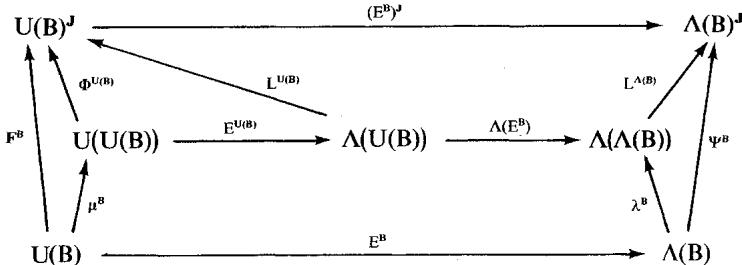
\includegraphics[keepaspectratio]{images/part001_4bd4d5b0.jpg}}

其中所有水平映射都是双射。）

\begin{enumerate}
\def\labelenumi{\alph{enumi})}
\setcounter{enumi}{1}
\item
  设 A 是一个预 λ -环。对每个 \(n \in \mathbf{J}\)，\(\psi_n\) 是 A 的加法群的一个自同态，且 \(\psi_1 = \mathrm{Id}_A\)。若 A 是 λ -环，则 \(\psi_n\) 是环 A 的自同态，且有 \(\psi_n \circ \psi_m = \psi_{nm}\)（对 J 中任意 \(n\)、\(m\)）。此外，对每个素数 \(p\)，我们有 \(\psi_p(a) \equiv a^p\) mod. \(p\mathbf{A}\)（对所有 \(a \in \mathbf{A}\)）。（利用 \(\lambda: \mathbf{A} \to \Lambda(\mathbf{A})\) 的单射性以及 \(\psi_n^{\mathbf{A}} = \mathbf{F}_n\) 的类似性质。）
\item
  设 A 是一个加法群为 Z -无挠的预 λ -环。为使 A 是一个 λ -环，必要且充分的是下列条件对满足 \(n \geqslant 2\) 与 \(m \geqslant 2\) 的所有整数成立：
\end{enumerate}

\begin{enumerate}
\def\labelenumi{(\roman{enumi})}
\item
  \(\psi_n(1) = 1\) ;
\item
  \(\psi_{n}(ab) = \psi_{n}(a)\psi_{n}(b)\)（对 A 中任意 \(a,b\)）；
\item
  \(\psi_{n}\circ \psi_{m} = \psi_{nm}\)
\end{enumerate}

由于 L : Λ(A) → A \(^{J}\) 是单射环同态，Ψ = L ∘ λ 是环同态当且仅当 λ 是环同态。对下图作同样的推理。

\pandocbounded{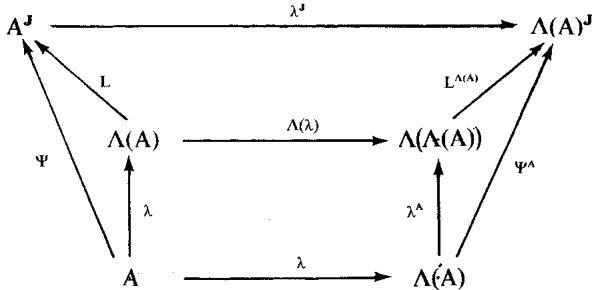
\includegraphics[keepaspectratio]{images/part001_ba507c2f.jpg}}

我们推出

\(\Lambda (\lambda)\circ \lambda = \lambda^{\mathbf{A}}\circ \lambda\)（λ 是 λ -态射）

\(\Leftrightarrow \lambda^{\mathbf{J}}\circ \Psi = \Psi^{\mathbf{A}}\circ \lambda \Leftrightarrow \lambda \circ \psi_{n} = \psi_{n}^{\mathbf{A}}\circ \lambda\)（对每个 \(n\)）

\(\Leftrightarrow \mathrm{L} \circ \lambda \circ \psi_n = \mathrm{L} \circ \psi_n^{\mathrm{A}} \circ \lambda\)（对每个 \(n\)）。

现在 \(\mathrm{L}\circ \lambda = \Psi\) 且 \(\mathbf{L}\circ \psi_n^{\mathbf{A}} = \mathbf{L}\circ \mathbf{F}_n = f_n\circ \mathbf{L}.\) 因此，

\(\Lambda (\lambda)\circ \lambda = \lambda^{\mathrm{A}}\circ \lambda \Leftrightarrow \Psi \circ \psi_{n} = f_{n}\circ \Psi\)（对每个 \(n\)）

\(\Leftrightarrow \psi_{m} \circ \psi_{n} = \psi_{nm}\)（对任意 \(m\) 与 \(n\)）。

\begin{enumerate}
\def\labelenumi{\alph{enumi})}
\setcounter{enumi}{3}
\tightlist
\item
  设 A 是一个 λ -环。设 \(a \in \mathbf{A}\) 是 λ -秩 \(\leqslant 1\) 的元素（即 \(\lambda(a) = 1 + a\mathbf{T}\)）。则有 \(\psi_n(a) = a^n\)（对所有 \(n \in \mathbf{J}\)）。若 P 是 A 的一个由 λ -秩 \(\leqslant 1\) 的元素组成的乘法子集，且 \(a_1, \ldots, a_r\) 属于 P，则我们有 \(\psi_n(a_1 + \cdots + a_r) = a_1^n + \cdots + a_r^n\)。
\end{enumerate}

在多项式代数 \(\mathbf{Z}[(\mathbf{X}_{i})_{i\in I}]\) 中，用 \((s_{n})\) 表示初等对称多项式 \(\sum_{n\geq0}s_{n}\mathbf{T}^{n}=\prod_{i}(1+\mathbf{X}_{i}\mathbf{T})\)，以及

\[
\mathrm{v} _ {n} (s _ {1}, \dots , s _ {n}) = \sum_ {i} \mathrm{X} _ {i} ^ {n}
\]

第 n 个 Newton 多项式。证明对任意 \(a \in A\)，有

\[
\psi_ {n} (a) = v _ {n} \left(\lambda_ {1} (a), \dots , \lambda_ {n} (a)\right).
\]

（首先当 \(a\) 是上述形如 \(a_{1} + \cdots + a_{r}\) 的元素时验证此关系。由此过渡到 \(a = 1 + \sum_{h \geqslant 1} s_{h} \mathrm{T}^{h} \in \Lambda(\mathbf{Z}[(\mathrm{X}_{i})_{i \in I}])\) 的情形。然后，把 A 嵌入 \(\lambda\) -环 \(\Lambda(\mathbf{A})\)，并利用同态 \(\mathbf{Z}[(s_{h})_{h=1,\ldots,n}] \to \mathbf{A}\)——它把 \(s_{h}\) 映为 \(\lambda_{h}(a)\)——推出一般情形。）

\begin{enumerate}
\def\labelenumi{\arabic{enumi})}
\setcounter{enumi}{48}
\tightlist
\item
  设 A 是一个环，E 是一个有限生成投射 A -模，且 \(u \in \text{End}_{\mathbf{A}}(\mathbf{E})\)。若 E 是自由 A -模，我们用 \(\det_{\mathbf{E}}(u)\) 表示 \(u\) 的行列式。一般地，可以选取一个 A -模 F 使得 \(\mathbf{E} \oplus \mathbf{F}\) 是一个有限生成自由 A -模，我们令
\end{enumerate}

\[
\det _ {E} (u) = \det _ {E \oplus F} (u \oplus 1 _ {F}).
\]

\begin{enumerate}
\def\labelenumi{\alph{enumi})}
\tightlist
\item
  证明 \(\operatorname{det}_{\mathbf{E}}(u)\) 与 F 的选取无关，\(\operatorname{det}_{\mathbf{E}}(1_{\mathbf{E}}) = 1\)，且有 \(\operatorname{det}_{\mathbf{E}}(u \circ v) = \operatorname{det}_{\mathbf{E}}(u) \cdot \operatorname{det}_{\mathbf{E}}(v)\)（对任意 \(u, v\)，在 \(\operatorname{End}_{\mathbf{A}}(\mathbf{E})\) 中）。
\end{enumerate}
